	\documentclass[10pt,oneside]{CBFT_book}
	% Algunos paquetes
	\usepackage{amssymb}
	\usepackage{amsmath}
	\usepackage{graphicx}
	\usepackage{libertine}
% 	\usepackage[bold-style=TeX]{unicode-math}
	\usepackage{lipsum}

	\usepackage{natbib}
	\setcitestyle{square}

	\usepackage{polyglossia}
	\setdefaultlanguage{spanish}


	\usepackage{CBFT.estilo} % Cargo la hoja de estilo

	% Tipografías
	% \setromanfont[Mapping=tex-text]{Linux Libertine O}
	% \setsansfont[Mapping=tex-text]{DejaVu Sans}
	% \setmonofont[Mapping=tex-text]{DejaVu Sans Mono}

	%===================================================================
	%	DOCUMENTO PROPIAMENTE DICHO
	%===================================================================

\begin{document}

\chapter{Ecuaciones de Hamilton-Jacobi}


\section{Introducción a la formulación de Hamilton}

Un sistema mecánico está caracterizado por $\{ q_i, \dot{q}_i \}$ las cuales dan un estado posible del sistema, y además
dan toda la información dinámica del mismo.

Ahora se describirá al sistema en términos de $ q_i, p_i \equiv \partial\Lag/\partial\dot{q}_i$  que tiene la característica
de producir una simetría en la mecánica así definida (la mecánica hamiltoniana).
La simetría es tal que son intercambiables $q_i$ y $p_i$.

Para las ecuaciones de movimiento se parte del hamiltoniano
\[
	\Ham = \sum_i p_i \dot{q}_i - \Lag( q_i, \dot{q}_i, t ),
\]
donde $\Ham =\Ham(q_i,p_i,t)$ tiene la misma información que $\Lag=\Lag(q_i,\dot{q}_i,t)$.

Se puede hacer una analogía con la termodinámica, pues la primer ley se escribe
\[
	dE = dQ - dW = \left. \dpar{E}{S} \right|_V dS - \left. \dpar{E}{V} \right|_S dV,
\]
lo cual implica que usando $S,V$ tengo como ``potencial'' a la energía.
Un estado termodinámico se define por dos variables; $(S,V), (T,P), (S,P), (T,V)$ que son cada par variables conjugadas.

Para definir estos potenciales se usan transformadas de Legendre. Así,
\[
	d(E-TS) = TdS -PdV - TdS -SdT = -PdV - SdT \equiv dA
\]
siendo $A$ la energía libre de Helmholtz.
\[
	d(E+PV) = TdS -PdV + PdV + VdP = TdS + VdP \equiv dH
\]
siendo $H$ la entalpía.

En el caso del Hamiltoniano se tiene 
\[
	d\Ham = \sum_i \dot{q}_i dp_i  + \sum_i p_i d\dot{q}_i - \sum_i \dpar{\Lag}{q_i} dq_i -
	\sum_i d \dpar{\Lag}{\dot{q}_i}\dot{q}_i - \dpar{\Lag}{t}dt 
\]
la cual usando las ecuaciones de Euler-Lagrange y el hecho de que $\partial{\Lag}/\partial{\dot{q}_i} $ es el momento conjugado
$p_i$ se tiene 
\[
	d\Ham = \sum_i \dot{q}_i dp_i  - \sum_i \dot{p}_i dq_i - \dpar{\Lag}{t}dt 
\]
y como esta ecuación es el diferencial total del hamiltoniano se tiene que
\[
	\dpar{\Ham}{t} = -\dpar{\Lag}{t} = \dtot{\Ham}{t}
\]
siendo la última igualdad una derivación vista oportunamente. Asimismo,
\[
	\dpar{\Ham}{p_i} = \sum_i \dot{q}_i \qquad \qquad 
	\dpar{\Ham}{q_i} = -\sum_i \dot{p}_i
\]
que son una mayor cantidad de ecuaciones pero de orden uno (comparando con las ecuaciones del sistema en el formalismo 
lagrangiano).

Con esto definimos un espacio de fases $(p_i,q_i)$ de $2N$ dimensiones para estudiar el movimiento de un sistema de partículas.
En el caso particular de una única partícula tendremos dos variables, $(p,q)$.

\subsection{La idea de Hamilton-Jacobi}

La idea es que se busca una transformación canónica que me transporte a un hamiltoniano nuevo donde toda la solución son 
constantes. Es decir 
\[
	H(q_i,p_i) \longrightarrow K(Q_i,P_i),
\]
donde
\be
	q_i \longrightarrow Q_i \equiv \beta_i \qquad p_i \longrightarrow P_i \equiv \alpha_i
	\label{coord_hamjac}
\ee
% para $\alpha,\beta$ constantes.
Pasamos a unas nuevas coordenadas y momentos $(\beta_i,\alpha_i)$ que son constantes. 
Aunque esto requiere conocer el problema (su solución). Esta transformación existe porque es ir atrás en el tiempo;
la antievolución.

Supongamos una generatriz del tipo $F_2 = S$, llamada {\it función principal de Hamilton}
\[
	S = S(q_i, \alpha_i, t).
\]
Entonces
\be
	\dpar{S}{q_i} = p_i \qquad \dpar{S}{\alpha_i} = \beta_i \qquad \dpar{S}{t} = H - K  
	\label{ecshamjac}
\ee
donde 
\[
	H(q_i,p_i,t) - \dpar{S}{t} = K = 0
\]
que es la condición necesaria para garantizar las condiciones \eqref{coord_hamjac}.
Esto lleva a la ecuación de Hamilton-Jacobi,
\be
	H(q_i,p_i,t) - \dpar{S}{t} = 0
	\label{ecshamjac2}
\ee
que no es otra cosa que una ecuación en derivadas parciales (PDE) al especializar $H$ en las derivadas parciales
\[
	H \left( q_i, \dpar{S}{q_i}, t \right) - \dpar{S}{t} = 0,
\]
que son $n+1$ variables y $n+1$ constantes (una es trivial porque la ecuación \eqref{ecshamjac2} no depende de $S$ sino de sus 
derivadas).

\begin{ejemplo}{\bf ejemplito}
\[
	H = \frac{p^2}{2m} + V(q)
\]
\[
	\frac{1}{2m} \Dpar{S}{q}^2 + V(q) + \dpar{S}{t} = 0
\]
hay que resolverlo utilizando condiciones iniciales
\[
	H(q_i,p_i,t) \qquad p_i(t=0) \qquad q_i(t=0).
\]
\end{ejemplo}

Notemos que 
\[
	\dpar{S}{q_i} = p_i(q_i,\alpha_i,t) \qquad \dpar{S}{\alpha_i} = \beta_i(q_i,\alpha_i,t)
\]

Cuando la ecuación es separable se puede garantizar la solución de Hamilton-Jacobi.
Si $H=H(q_i,\alpha_i)$, el hamiltoniano no depende del tiempo, entonces $dH/dt = \partial H/\partial t=0$ y en ese caso es 
$H=cte.$ (la energía). Se tiene
\[
	H \left( \dpar{S}{q_1},...,\dpar{S}{q_N},q_1,...,q_N \right) + \dpar{S}{t} = 0, 
\]
o bien
\[
	\dpar{S}{t} = -E,
\]
por lo tanto es separable en el tiempo. Entonces
\[
	S = W(q_1,...,q_N,\alpha_1,...,\alpha_N) - E t,
\]
donde $W$ no depende del tiempo, que sólo aparece explícito en el segundo término. Luego
\[
	\dpar{S}{q_i} = \dpar{W}{q_i}
\]
con lo cual 
\[
	H \left( \dpar{W}{q_1},...,\dpar{W}{q_N},q_1,...,q_N \right) = E
\]
y tengo un nuevo hamiltoniano que no vale cero sino que vale $E$.
Pase a {\it un lugar} donde los momentos son constantes y las coordenadas son cíclicas.
\[
	E = E(\alpha_1, ..., \alpha_N )
\]
de manera que $\partial E/\partial \alpha_N = a$ y luego,
\[
	Q = at + Q_0 \qquad \text{ las $Q$ son lineales}
\]
Entonces,
\[
	\dpar{E}{\alpha} = \dot{Q} = a \qquad \text{ una constante}
\]
y
\[
	\dpar{E}{p} = \dpar{E}{\alpha} = \dot{Q}.
\]

Remarquemos que si fuera $E=E(q)$ entonces $\partial E \ \partial q = \dot{\alpha}$ y no sería constante $\alpha$, pero $E$ no 
depende de $Q_i$.

\begin{ejemplo}{\bf Ejemplito de un grado de liberad}

\[
	H = \frac{p^2}{2m} + V(q) \qquad \qquad S = W - Et
\]
\[
	E = \frac{1}{2m} \Dtot{W}{q}^2 + V(q), 
\]
de modo que 
\[
	\dtot{W}{q} = \pm \sqrt{2m[E-V(q)]},
\]
\[
	W(q,E) = \pm \int \sqrt{2m[E-V(q)]} dq - Et
\]

Para un grado de libertad siempre tendrá esta forma.
\end{ejemplo}

Para más grados de libertad deberíamos poder separar alguna coordenada en igual forma. Si $q_1$ no aparece, entonces la derivada 
del hamiltoniano $H$ respecto a $q_1$ dice que será constante el $\dot{q}_1$, es decir
\[
	\dpar{W}{q_1} = \alpha_2 \quad \to \quad 
	H\left( \alpha_2, \dpar{W}{q_2},...,\dpar{W}{q_N},q_2,...,q_N \right) = E.
\]

Es más, si la $S$ es totalmente separable de la forma 
\[
	S(q_i,\alpha_0) = \sum_{i=1}^N \; W_i(q_i,\alpha_1,...,\alpha_N) - Et
\]
lo cual, dicho sea de paso, requerirá $N$ constantes de movimiento, entonces se puede resolver completamente.

[Lo que sigue es un refrito de lo anterior o viceversa; habría que consolidarlo]
[...] y podemos poner $H=\alpha_1$.
Entonces
\[
	\dpar{S}{t} = -\alpha_1 \quad \longrightarrow \quad S=W(q_i,\dpar{S}{q_i}) -\alpha_1 t .
\]

Se procede en la misma forma con cada coordenada hasta obtener $S$.

Podemos ver que si $\alpha_1 = \alpha_1(\alpha_i)$, y me quedo con $H=\alpha_1 \equiv K$ entonces
\[
	\dpar{K}{\alpha_i} = a = \dot{Q}_i \longrightarrow Q_i = \beta = a t + \beta_0 
\]
\[
	\dpar{K}{\beta_i} = 0 = -\dot{P}_i \longrightarrow P_i = \alpha_i (ctes.).
\]

La $\alpha_1$ no puede depender de $q_i$ pues si se tuviera $\partial \alpha_1 /\partial q_i \neq 0$ 
no sería constante $\alpha_1$ pues $\dot{q}\neq 0$.

Luego, invirtiendo las ecuaciones \eqref{ecshamjac} determinamos las trayectorias
\[
	q_i = q_i(\alpha_i, \beta_i, t).
\]

Además, si el problema es totalmente separable, entonces
\[
	S = \sum_i^N \; W(q_i, \alpha_1,...,\alpha_n) - \alpha_1 t
\]
y tendré tantas constantes de movimiento como grados de libertad. La solución se compone de problemas
independientes en una variable.

% =================================================================================================
\section{Preservación del volumen en una transformación canónica}
% =================================================================================================

Definamos un hipervolumen $\mathcal{V}$ en el espacio de fases de acuerdo a
\[
	\int dq_1 dq_2 ... dq_n dp_1 dp_2 ... dp_n = \mathcal{V}_{p,q}
\]
que en otras coordenadas es
\[
	\int dQ_1 dQ_2 ... dQ_n dP_1 dP_2 ... dP_n = \mathcal{V}_{P,Q}.
\]

\begin{figure}
	\begin{center}
	\includegraphics[width=0.4\textwidth]{images/fig_mc_hamjac2.pdf}	 
	\end{center}
	\caption{}
\end{figure} 

El jacobiano de la transformación, que permite convertir una integral en la otra, es 
\[
	\frac{\partial (Q_1,...,Q_n,P_1,...,P_n)}{\partial (q_1,...,q_n,p_1,...,p_n)} 
\]
y puede verse que vale 1. En efecto, como vale una especie de {\it chain rule}
\[
	\frac{\partial (Q_1,...,Q_n,P_1,...,P_n)}{\partial (q_1,...,q_n,p_1,...,p_n)}  =
	\frac{\partial (Q_1,...,Q_n,P_1,...,P_n)/\partial (q_1,...,q_n,P_1,...,P_n)|_{P_i=cte}}
	{\partial (q_1,...,q_n,p_1,...,p_n)/\partial (q_1,...,q_n,P_1,...,P_n)|_{q_i=cte}}
\]

El jacobiano en notación matricial es 
\[
	\begin{pmatrix}
	\dpar{Q_1}{q_1} & \dpar{Q_1}{q_2} & ... & \dpar{Q_1}{p_n} \\
	.. & .. & .. & .. \\
	\dpar{P_n}{q_1} & .. & .. & \dpar{P_n}{p_n}
	\end{pmatrix}
\]
Entonces se puede ver que para el numerador es
\[
	J_{ij}^{num} = \dpar{Q_i}{q_j} = \frac{\partial}{\partial q_j} \left(\dpar{F_2}{P_i} \right)
\]
mientras que para el denominador,
\[
	J_{ij}^{den} = \dpar{p_i}{P_j} = \frac{\partial}{\partial P_j} \left(\dpar{F_2}{q_i} \right)
\]
pero como estas dos expresiones son iguales se tiene que $J=1$ y entonces se conserva
el volumen, aunque cambiando de forma (se deforma la cáscara pero el volumen se conserva).

Usando $|M| = |M^t|$ entonces se ve que vale uno el cociente de los jacobianos. Siempre y cuando sea
la transformación canónica.

Son invariantes canónicos
\[
	\int\int \sum_{i=1}^N \; dq_i dp_i \qquad \qquad  \int\int \sum_{j=1}^N \sum_{i=1}^N \; dq_i dp_i dq_j dp_j
\]

En sistemas de un grado de libertad
\[
	A_{p,q} = \int dp dq \qquad A_{P,Q} = \int dP dQ
\]
y el jacobiano
\[
	J = \begin{vmatrix}
	     \dpar{Q}{q} & \dpar{Q}{p} \\
	     \dpar{P}{q} & \dpar{P}{p}
	    \end{vmatrix} =
	    \dpar{Q}{q} \dpar{P}{p} - \dpar{Q}{p} \dpar{P}{q} = [Q, P] = 1.
\]
\begin{figure}[!h]
	\begin{center}
	\includegraphics[width=0.6\textwidth]{images/fig_mc_hamjac1gl.pdf}	 
	\end{center}
	\caption{}
\end{figure} 

Notamos que el jacobiano en una transformación canónica para un sistema de un grado de libertad es el corchete de Poisson 
de $Q,P$, y además da uno. El área se conserva.

Comentemos que un sistema disipativo achica el área de la transformación.

En la transformación, el número de puntos en $p,q$  es el mismo en $PQ$ pero la forma que adopta varía. Es como un líquido
incompresible.

La transformación canónica cumple que, se parte de una punto a otro por una trayectoria que no corta con ninguna otra.

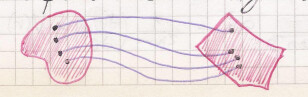
\includegraphics[width=0.6\textwidth]{images/fig_mc_espacio_fases.jpg}	

No confundir espacio de fases con espacio de configuración.

% =================================================================================================
\section{Variables ángulo-acción}
% =================================================================================================

La idea es introducir un nuevo juego de variables canónicas. Para ello consideremos una transformación 
canónica 
\[
	(p, q) \longrightarrow (J, \theta)
\]
con generatriz $W$ que cumple $W-Et=S$. 
Estas variables se pueden utilizar solamente con
\begin{itemize}
	\item Problemas conservativos, donde es $S = W - Et $
	\item Problemas completamente separables, con
	\[
		W = \sum_i^N \; W_i(q_1,\alpha_1,...,\alpha_n)
	\]
	\item Problemas de movimiento periódico (condicionalmente)
\end{itemize}

Solamente si se verifican estos tres supuestos, se pueden utilizar las variables $(J,\theta)$.

El movimiento periódico es de dos tipos, de rotación o libración,

% \begin{figure}[htb]
% 	\begin{center}
	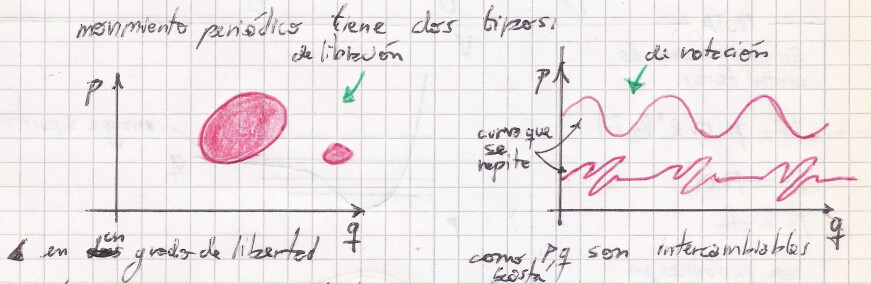
\includegraphics[width=0.7\textwidth]{images/fig_mc_rot_lib.jpg}	 
% 	\end{center}
% 	\caption{}
% \end{figure} 

Si tengo más de un grado de libertad tendré un gráfico $pq$ para cada par y puedo tener una
libración o una rotación (si el problema es separable). De lo contrario no podré expresar
cada $p$ en función de su $q$ correspondiente.

\subsection{Algunos claims sueltos}

Dado un problema puede ser conveniente pasar a un hamiltoniano $H'$ más sencillo, donde la relación
con el anterior es
\[
	H' = H + \dpar{S}{t},
\]
y si $S$ se elige del tipo $F_2$ se tiene $S = W - Et$. La $S$ depende de variables viejas y nuevas
(en mitades). El hamiltoniano más conveniente es $H'=0$
\[
	S = W_1(q_1, \alpha_1, ..., \alpha_n) + W_2(q_2, \alpha_1, ..., \alpha_n) - Et,
\]
y es tal que 
\[
	p = \dpar{S}{q} \qquad Q = \dpar{S}{\alpha} = B = cte
\]

Las integrales que son $W$ conviene esperar para primero derivarlo [?].
Ángulo-acción es un caso particular.
Necesito periodicidad de los grados de libertad (no de todos igual período a la vez).
La acción es $J$ y la tomamos como el nuevo momento,
\[
	J = \frac{1}{2\pi } \oint p dq,
\]
donde la integral se hace en un ciclo y el $2\pi$ está para que sea angular. Sin este factor será
la frecuencia natural. Entonces el hamiltoniano será la energía, $H=H'=E$ e ignoramos la parte
temporal.
\[
	\omega = \dpar{E}{J}
\]

Con esto ya obtenemos la frecuencia. Si queremos la solución completa habría que invertir.
La geometría da $p,q \to J,\theta$ es $W = \int pdq$ generatriz.
\[
	\theta = \dpar{W}{J} = \omega t + \theta_0.
\]

En el espacio de fases el área de una trayectoria está asociada con la generatriz

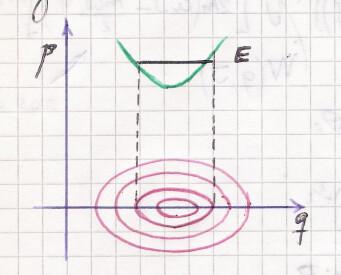
\includegraphics[width=0.5\textwidth]{images/fig_mc_angacc.jpg}

\begin{ejemplo}{\bf Partícula en un pozo de potencial}

Tenemos una partícula en un pozo de potencial

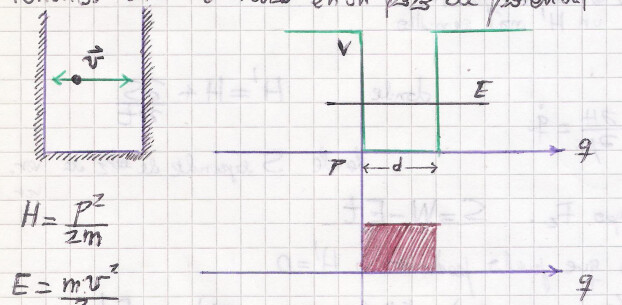
\includegraphics[width=0.5\textwidth]{images/fig_mc_angacc2.jpg}
 
Se tienen 
\[
	H = \frac{p^2}{2m} \qquad E = \frac{m v^2}{2} \qquad p = m v
\]
y entonces
\[
	J = \frac{1}{\pi} \int \sqrt{2 m E} dq = \sqrt{2 m E} d,
\]
y como 
\[
	\omega = \frac{\pi p}{m d} = \frac{2\pi v}{2d}
\]
siendo el período $\tau = 2d/v$. Podemos conectar $E$ con $p$ a través de estas fórmulas.
Pasamos a un problema donde todas las coordenadas son cíclicas.
\[
	W = \int p dq = \begin{cases}
			\sqrt{ 2 m E } \; q = \frac{J \pi q}{d} \text{ ida } \\
			\\
			\sqrt{ 2 m E } \; ( d + d - q) = \frac{J \pi (2d-q)}{d} \text{ vuelta }
	                \end{cases}
\]
y
\[
	p = \dpar{W}{q} = \begin{cases}
			\sqrt{ 2 m E } \\
			\\
			-\sqrt{ 2 m E }
	                 \end{cases}
\]
\[
	\theta = \dpar{W}{J} = \begin{cases}
	                        \frac{\pi q}{d} \\
	                        \\
	                        \frac{\pi}{d}(2d-q)
	                       \end{cases}
\]
que conducen a
\[
	q = \begin{cases}
		\frac{d}{\pi} ( \omega t + \theta_0 ) \\
		\\
		2d - \frac{d}{\pi} ( \omega t + \theta_0 )
	    \end{cases}
\]
 
\end{ejemplo}


\subsection{Péndulo}

La energía en el caso del péndulo es
\[
	E = \frac{p^2}{2m} + m g \ell ( 1 - \cos q )
\]
y un grado de libertad es separable siempre si se conserva la energía.
El péndulo realiza dos movimientos,
\[
	E > 2mg\ell \quad \text{ rotación} \qquad \qquad E < 2mg\ell \quad \text{ libración}
\]

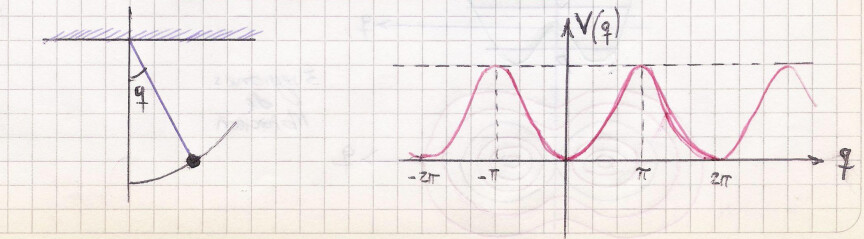
\includegraphics[width=0.7\textwidth]{images/fig_mc_pendulo_angacc1.jpg}

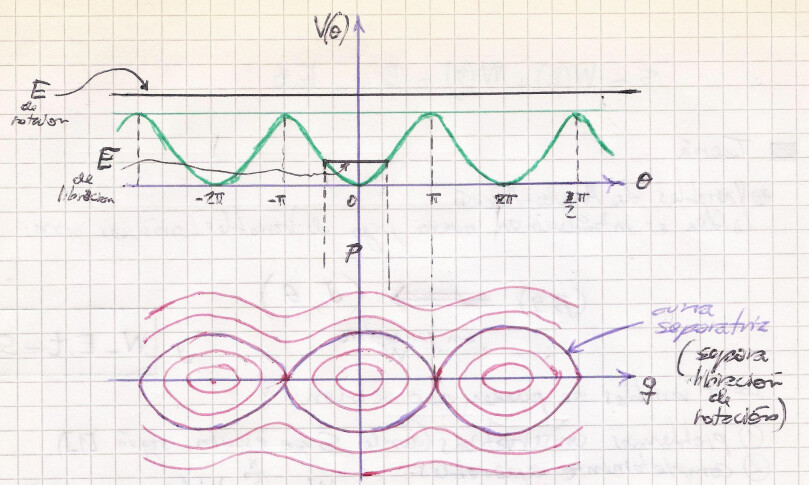
\includegraphics[width=0.7\textwidth]{images/fig_mc_pendulo_angacc2.jpg}

En un sistema con varios grados de libertad, cada grado de libertad deberá tener un grafo de
esta forma.
Se ve que para pequeñas apartaciones $q$ es
\[
	E \approx \frac{p^2}{2m} + \frac{ m g \ell q^2 }{2},
\]
lo cual no es otra cosa que el gráfico de una elipse. Luego, será una elipse {\it toda la vida} mediante
suma de pequeños desplazamientos (perturbaciones). La idea es, entonces, que no podemos pasar de una
libración a una rotación mediante perturbaciones pequeñas. 
Libración y rotación son dos movimientos de naturaleza diferente.
No se puede atravesar la separatriz perturbando una solución de un movimiento.

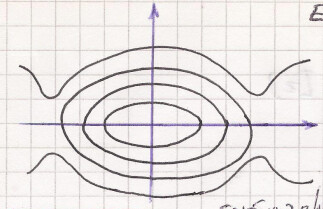
\includegraphics[width=0.3\textwidth]{images/fig_mc_pendulo_angacc3.jpg}

La integral de acción es
\[
	J_i = \frac{1}{2\pi}\int_{ciclo} p_i(q_1,\alpha_1,...,\alpha_n) dq_i
\]
donde 
\[
	J_i = J_i(\alpha_1,...,\alpha_n)
\]
son los nuevos momentos, constantes, y a su vez los $\alpha_i$ son constantes de separación.
Asimismo $\alpha_i=\alpha_i(J_1,...,J_n)$. Una integral de acción para cada grado de libertad.
Esta integral las puedo hacer siempre dadas las condiciones que se supusieron.

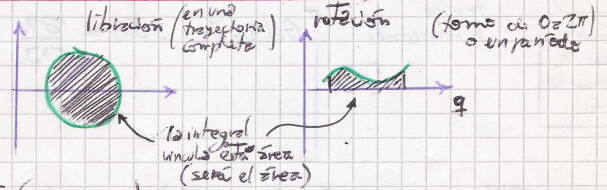
\includegraphics[width=0.8\textwidth]{images/fig_mc_pendulo_angacc4.jpg}

\begin{ejemplo}{\bf Comentario central forces}

En un problema de fuerzas centrales, por ejemplo, se tienen
\[
	p_r = p_r(r,\ell^2,\ell_z,E) \qquad p_\vp = p_\vp(\vp) \quad p_\theta =cte
\]
que son periódicas en cada coordenada pero no el movimiento total porque en general
no coinciden los períodos de todos los movimientos en $r,\theta,\phi$.
Es decir, que la a periodicidad de cada coordenada no implica periodicidad de todo el movimiento real.

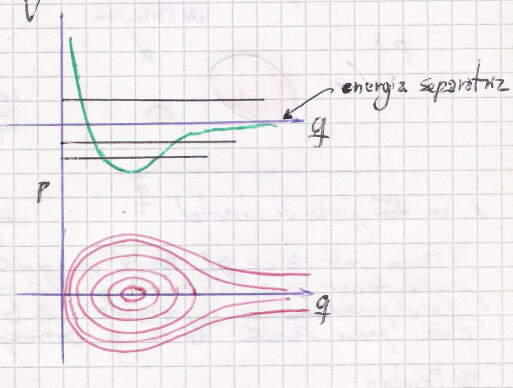
\includegraphics[width=0.7\textwidth]{images/fig_mc_pendulo_angacc5.jpg}

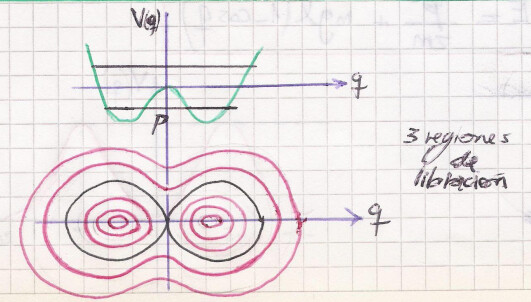
\includegraphics[width=0.7\textwidth]{images/fig_mc_pendulo_angacc6.jpg}

\end{ejemplo}

\subsection{Oscilador armónico}

La energía es
\[
	E = \frac{p^2}{2m} + \frac{1}{2} m \omega^2 q^2
\]
 
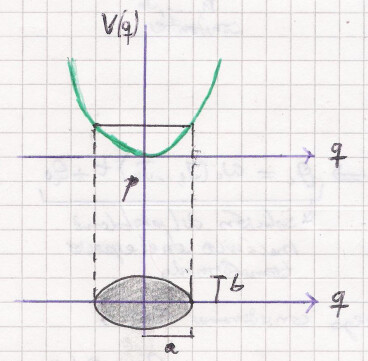
\includegraphics[width=0.5\textwidth]{images/fig_mc_osciladorarm_angacc.jpg}

de manera que
\[
	1 = \frac{p^2}{2mE} + \frac{m\omega^2 q^2}{2E}
\]
y
\[
	J = \frac{1}{2\pi}(\pi a b )= \frac{E}{\omega}.
\]

Para el oscilador armónico es entonces
\[
	\dpar{E}{J} = \dot{\theta}
\]
y luego
\[
	\theta = \omega t + \theta_0
\]
de modo que 
\[
	E = E(J_1, J_2, ..., J_n)
\]
siempre puedo despejar $E$ en función de los nuevos momentos.
\[
	\dpar{E}{J_i} = \dot{\theta}_i = \omega_i(J_1,...,J_n)
\]
\be
	\theta_i = \omega_i(J_1,...,J_n) t + \theta_0
	\label{sol_theta}
\ee
y habrá órbitas cerradas dependiendo de las condiciones iniciales de los $J_i$.
Ahora faltaría obtener los $q(t),p(t)$ a partir de la  \eqref{sol_theta}. Sabemos que 
\[
	W = \sum_i^N W_i(q_i,\alpha_1,...,\alpha_n),
\]
la generatriz total es una suma y los $\alpha_i$ son las constantes de separación. Necesito
\[
	W = W( q_i, J_1, ..., J_n ).
\]

Utilizo $\alpha_i( J_1, J_2, ..., J_n )$ (que se obtuvieron de las $n$ integrales de acción) y $\partial W /\partial J_i = \omega_t t + \theta_0 $.
Luego tendré $n$ relaciones del tipo
\be
	\theta_i( q_i, J_1, ..., J_n ) = \dpar{\theta}{J_i} = \omega_i t + \theta_0
	\label{sistema_theta}
\ee
y $n$ ecuaciones 
\[
	\dpar{W_i}{q_i} = p_i = p_i( q_i, J_1, ..., J_n ) 
\]
usando condiciones iniciales $(q_1, ..., q_n), (p_1, ..., p_n)$ en $t=0$ especializando a $t=0$ obtengo $J_1, ..., J_n$ constantes.
\[
	W = \sum_i^N \; W_i(q_i,J_1,...,J_n). 
\]

En el sistema \eqref{sistema_theta} con la $E$ hago 
\[
	\dpar{E}{J_i}(J_1,...,J_n) = \dot{\theta}_i(J_1,...,J_n)
\]
entonces $\theta_i = \omega_i (J_1,...,J_n) t + \theta_0$ que es la solución del problema en el espacio mecánico transformado.
Los $J_1,...,J_n$ son constantes porque dependen de constantes $\alpha_i$ .

Luego, consideramos $t=0$ y $\theta_i = \theta_i ( q_1,...,q_n,J_1,...,J_n)$ provee los $q_i = q_i(t)$. Se tiene 
\[
	p_\ell = \dpar{W_\ell}{q_\ell} = p_\ell( q_\ell, J_1, ..., J_n ).
\]

Para el oscilador armónico
\[
	E = \omega J \qquad \qquad \theta = \omega t + \theta_0
\]
\[
	W(q,E) = \int \frac{dq}{ [ 2 m \left( E - \frac{1}{2} m \omega^2 q^2 \right) ]^{-1/2} } = 
	W(q,J) = \int \frac{dq}{ [ 2 m \left( \omega J - \frac{1}{2} m \omega^2 q^2 \right) ]^{-1/2} },
\]
donde el denominador contiene el $\acos$ de algo.
\[
	\dpar{W}{J}(q,J) = \theta (t) = \omega t + \theta_0 = \int \frac{ m \omega dq }{ [ 2 m \left( \omega J - \frac{ m \omega^2 q^2 }{2} \right) ]^{1/2} }
\]
y
\[
	\dpar{W}{q} = \sqrt{ \omega J - \frac{ m \omega^2 q^2 }{2} \left( \right) } = p.
\]

\subsubsection{Quedó remanente}

\begin{figure}
	\begin{center}
	\includegraphics[width=0.7\textwidth]{images/fig_mc_hamjac.pdf}	 
	\end{center}
	\caption{}
\end{figure} 


La transformación $S$ es 
\[
	\dpar{S}{q_i} = p_i = \dpar{W}{q_i} \qquad \dpar{S}{J_i} = \theta_i = \dpar{W}{J_i}
\]
siendo $p_i = p_i(q_1,J_1,...,J_n)$.
El nuevo hamiltoniano es $E=E(J_1,...,J_n)$
\[
	\dpar{E}{J_i} = \dot{\theta}_i \equiv \omega \qquad \dpar{E}{\theta_i} = -\dot{J}_i
\]
de manera que tenemos
\[
	\theta_i = \omega t + \theta_{0_i} \qquad  \dpar{W}{J_i} = \theta_i = \theta_i(q_i, J_i)
\]
y entonces despejamos las $q_i$ desde
\[
	\theta_i(q_i, J_i) = \omega t + \theta_{0_i}.
\]

Las condiciones iniciales $(q_i, J_i)$ se introducen en
\[
	\dpar{W}{q_i} = p_i(q_1,J_1,...,J_n)
\]
y obtengo las $J_1, ..., J_n$ constantes.

% =================================================================================================
\section{Transformación canónica infinitesimal}
% =================================================================================================

Difieren de la identidad en un infinitésimo
\[
	F_2 = 	F_2(q_i,P_i) = \sum_i^N q_iP_i
\]
es la identidad
\[
	\dpar{F_2}{q_i} =  p_i \equiv P_i \qquad \dpar{F_2}{P_i} =  Q_i \equiv q_i
\]
y donde considero
\[
	F_2(q_i,P_i) = \sum q_i P_i + \epsilon G(q_1,...,q_n,P_1,...,P_n) \qquad \textrm{con} \; \epsilon \ll 1
\]
\[
	\dpar{F_2}{q_i} = p_i = P_i + \epsilon\dpar{G}{q_i} \longrightarrow P_i = p_i - \epsilon\dpar{G}{q_i} 
\]
\[
	\dpar{F_2}{P_i} = Q_i = q_i + \epsilon\dpar{G}{P_i} \longrightarrow q_i = Q_i - \epsilon\dpar{G}{P_i} 	
\]
donde $\partial G/\partial P_i \approx \partial G/\partial p_i$ diferirán en un orden $\epsilon^2$ el cual
descarto. Entonces
\[
	\delta p_\ell = -\epsilon \dpar{G}{q_\ell} \qquad \delta q_\ell = \epsilon \dpar{G}{P_\ell}.
\]

Si considero $H$ en lugar de $G$ y $\epsilon = \delta t$ entonces
\[
	\frac{\delta p_\ell}{\delta t} = -\dpar{H}{q_\ell} \qquad \frac{\delta q_\ell}{\delta t} = \dpar{H}{p_\ell}
\]
de tal manera que 
\[
	\dot{p}_\ell = -\dpar{H}{q_\ell} \qquad \dot{q}_\ell = -\dpar{H}{p_\ell}
\]
y donde se ve que el $H$ genera la transformación evolución temporal.
Por otra parte, se puede ver cómo varía una cierta cantidad $A$ ante la transformación canónica.
\[
	\delta A = A(q_i + \delta q_i, p_i + \delta p_i) - A(q_i,p_i)
\]
y
\[
	\delta A = \sum_i \left( \dpar{A}{q_i} \delta q_i + \dpar{A}{p_i} \delta p_i \right)
\]
\[
	\delta A = \epsilon \sum_i \left( \dpar{A}{q_i} \dpar{H}{p_i} - \dpar{A}{p_i} \dpar{H}{q_i} \right) =
	\epsilon[A,H] \longrightarrow \frac{\delta A}{\delta t} = [A,H]
\]
entonces las constantes de movimiento generan transformaciones canónicas infinitesimales que dejan invariante
al hamiltoniano $H$. Si
\[
	\dtot{A}{t} = 0 \Longrightarrow [A,H] = 0
\]

Consideremos una rotación infinitesimal. Una rotación en torno al eje $z$
\[
	\begin{cases}
		x_i' = x_i - \delta \alpha y_i \\
		y_i' = y_i + \delta \alpha x_i \\
		z_i' = z_i
	\end{cases}
\]
que implica 
\[
	\delta x_i = -  \delta \alpha y_i \qquad \qquad \delta y_i = \delta \alpha x_i \qquad \qquad 
	\delta z_i = 0
\]
\notamargen{Las constantes de movimiento están generadas por simetrías (Noether).}

Luego,
\[
	G = \sum_i ( x_i p_{y_i} - y_i p_{x_i} ) = \ell_z
\]
y una rotación en torno a $\hat{n}$ es
\[
	\delta\alpha [ A, \vb{L}\cdot\vb{n} ] = \delta A,
\]
si $A$ es un vector $\vb{V}$ entonces
\[
	\delta\alpha [ \vb{V}, \vb{L}\cdot\vb{n} ] = \delta \vb{V} = \delta\alpha \vb{n} \times \vb{V},
\]
de modo que 
\[
	[ \vb{V}, \vb{L}\cdot\vb{n} ] = \vb{n} \times \vb{V}
\]
es una relación vectorial; es decir que valen
\[
	[ V_x, \vb{L}\cdot\vb{n} ] = (\vb{n} \times \vb{V})_x
\]
y lo mismo para los componentes $y,z$. Además
\[
	[L_x, L_z] = ( \hat{z} \times \vb{L} )_z = - L_y
\]
\[
	[L_y, L_z] = ( \hat{z} \times \vb{L} )_y = L_x
\]
\[
	[L_x, L_y] = ( \hat{y} \times \vb{L} )_x = L_z
\]
o bien 
\[
	[L_i, L_j] = \varepsilon_{ijk} L_k
\]
donde 
\[
	\varepsilon_{ijk} = \begin{cases}
	 0 \quad \text{ si se repite índice } \\
	 1 \quad \text{ si es permutación cíclica } \\
	 -1 \quad \text{ si es permutación anticíclica }
	\end{cases}
\]

Esto nos dice que no podemos elegir como momentos estas constantes de movimiento puesto que el
corchete de Poisson entre ellas es nulo.
No va a existir transformación canónica donde $p_1 = L_x, p_2 = L_y, p_3 = Lz$ pues su corchete de
Poisson entre ellas no se anula.

% =================================================================================================
\section{Volviendo a Hamilton-Jacobi}
% =================================================================================================

\be
	H\left( \dpar{S}{q_1}, ..., \dpar{S}{q_n}, q_1, ..., q_n, t \right) - \dpar{S}{t} = 0
	\label{ham-jac}
\ee
y se pasaba de coordenadas $q,p$ a constantes $\alpha,\beta$.

Lo único que se puede asegurar son condiciones para hallar solución a \eqref{ham-jac} pero no resolverla.
La condición es que \eqref{ham-jac} sea separable, que existan tantas constantes de movmiento como grados
de libertad. Si el hamiltoniano tiene alguna coordenada cíclica o no depende del tiempo entonces se podría
separar, pero en general no es el caso.

Podría suceder que
\[
	W = \sum_{i=1}^N W_i(q_i,\alpha_1,...,\alpha_N)
\]
y entonces no podré llegar a una solución que se compone de problemas independientes en una variable.

En fuerzas centrales tenemos un ejemplo. Escribamos
\[
	H = \frac{p_r^2}{2m} + \frac{p_\vp^2}{2mr^2\sin^2\theta} + \frac{p_\theta^2}{2mr^2} + V(r) = E
\]
y
\[
	W = W_r(r,\alpha_1,\alpha_2,\alpha_3) + W_\vp(\vp,\alpha_1,\alpha_2,\alpha_3) + 
		W_\theta(\theta,\alpha_1,\alpha_2,\alpha_3)
\]
donde
\[
	\frac{1}{2m} \Dtot{W_r}{r}^2 + \frac{1}{2mr^2} \Dtot{W_\theta}{\theta}^2 + \frac{1}{2mr^2\sin^2\theta} \Dtot{W_\vp}{\vp}^2
	+ V(r)  = E \equiv \alpha_1
\]
y siendo que $E$ es una constante, la denominamos $\alpha_1$.

Luego, como en 
\[
	\left[\frac{1}{2m} \Dtot{W_r}{r}^2 + \frac{1}{2mr^2} \Dtot{W_\theta}{\theta}^2 + V(r) - \alpha_1 \right] 
	2 m r^2 \sin^2\theta = - \Dtot{W_\vp}{\vp}^2
\]
el miembro izquierdo sólo depende de $r,\theta$ y el derecho de $\vp$ tienen que ser una constante ambos
miembros.

Asimismo,
\[
	\dtot{W_\vp}{\vp} = \alpha_2,
\]
y $W_\vp = \alpha_2 \vp$ porque $\vp$ es cíclica en fuerzas centrales. Es más, $\alpha_s$ es el momento angular
en $z$ ($L_z$, que es constante).
Entonces
\[
	\frac{1}{2m} \Dtot{W_r}{r}^2 + \frac{1}{2mr^2} \:
	\left[ \frac{\alpha_2^2}{\sin^2\theta} + \Dtot{W_\theta}{\theta}^2 \right]  + V(r) = \alpha_1,
\]
donde el corchete será $\alpha_3^2$. Ahora puedo separar otra vez y surge $\alpha_3^2$ que será el $|\vb{L}|^2$ total.
Las $\alpha_i$ son constantes de separación.
Si hubiese escrito con $\theta = \pi / 2$ entonces resultaba más detectable.
\[
	W(\theta) = \int \sqrt{ \left( \alpha_3^2 - \frac{\alpha_2^2}{\sin^2\theta} \right) } \; d\theta
\]
y luego
\[
	\frac{1}{2m} \Dtot{W_r}{r}^2 + \frac{1}{2mr^2} \: \alpha_3^2 + V(r) = \alpha_1
\]
al solucionar lo anterior
\[
	W_r = \int \sqrt{ 2 m ( \alpha_1 - V(r) - \alpha_2^2 / (2mr^2) ) } \; dr
\]
y el nuevo hamiltoniano es $ K = \alpha_1 $. Entonces
\[
	\dpar{K}{\alpha_2} = 0 \qquad \text{ que lleva a } \qquad \beta_2 = cte.
\]
\[
	\dpar{K}{\alpha_3} = 0 \qquad \text{ que lleva a } \qquad \beta_3 = cte.
\]
\[
	\dpar{K}{\alpha_1} = 1 \qquad \text{ que lleva a } \qquad \beta_2 = t + \beta_{10}
\]
Como
\[
	\dpar{W}{\alpha_1} = \dpar{W_r}{\alpha_1}
\]
se tiene 
\[
	\beta_1 = \int \frac{m}{\sqrt{ 2 m ( \alpha_1 - V(r) - \alpha_2^2 / (2mr^2) ) }} dr,
\]
que es igual a la ecuación ya calculada en el caso de fuerzas centrales.

La forma de separar también funciona si
\[
	V = V(r) + \frac{a(\vp)}{r^2 \sin ^2 \theta} + \frac{b(\theta)}{r^2},
\]
es decir, si el $V$ tiene una forma como la de arriba en coordenadas esféricas.

Consideremos unas coordenadas $\xi,\eta,\vp$ que se relacionan por
\[
	\rho = \xi \eta \qquad z = \frac{1}{2}( \xi - \eta ) \qquad \vp = \vp
\]
donde $\rho,z,\vp$ son las polares cilíndricas usuales.
Un potencial de la forma 
\[
	\frac{ a(\xi) + b( \eta ) }{ \xi + \eta }
\]
en coordenadas parabólicas puede separarse.

En coordenadas elípticas
\[
	\rho = \sigma \sqrt{ ( \xi^2 - 1 )( 1 - \eta^2 ) } \qquad z = \sigma \xi \eta \qquad \vp = \vp
\]
un potencial de la forma 
\[
	V = \frac{ a(\xi) + b( \eta ) }{ \xi^2 - \eta^2 }
\]
puede separarse.

En cartesianas es
\[
	V(\vb{x}) = A(x) + B(y) + C(z)
\]
condición suficiente de verificación para Hamilton-Jacobi. Si el potencial es separable entonces tengo tantas coordenadas como 
constantes de movimiento, entonces si tengo la solución [?].

\subsection{Comentario Schrödinger}

La ecuación de Schrödinger es
\[
	- \frac{\hbar^2}{2m} \nabla^2 \Psi(\vb{x},t) + V(r) \Psi(\vb{x},t) = i \hbar  \dpar{\Psi}{t} (\vb{x},t).
\]
Si ensayamos como solución 
\[
	\Psi(\vb{x},t) = b(\vb{x},t)  \euler^{i A(\vb{x},t) / \hbar},
\]
se tendrá 
\[
	b V(r) + \frac{b}{2m} \left[ \Dpar{A}{x}^2 + \Dpar{A}{y}^2 + \Dpar{A}{z}^2 \right] = - b \dpar{A}{t}
\]
o bien 
\[
	\frac{1}{2m} \left[ \Dpar{A}{x}^2 + \Dpar{A}{y}^2 + \Dpar{A}{z}^2 \right] + V(r) + \dpar{A}{t} = 0
\]

Ecuación de Hamilton-Jacobi (con igualar el orden cero)
\[
	\frac{1}{m} \Dpar{b}{x} \dpar{A}{x} + \frac{b}{2m} \dpar[2]{A}{x} = - \dpar{B}{t}
\]
\[
	\dpar{}{x}\left( b^2 \frac{1}{m} \dpar{S}{x} \right) + \dpar{b^2}{t} = 0
\]

Esto lleva a 
\[
	\nabla \left( \rho \frac{\vb{p}}{m} \right) + \dpar{\rho}{t} = 0,
\]
que es una ecuación de continuidad para la densidad de probabilidad.
De algún lado sacamos, por la situación estacionaria,
\[
	- \dpar{b}{x} \dpar{A}{x} = \frac{1}{2} \Dpar[2]{A}{x} b,
\]
que equivale a 
\[
	\frac{1}{b} \dpar{b}{x} = - \frac 1 2 \Dpar[2]{A}{x} \Dpar{A}{x}^{-1}
\]
o bien a 
\[
	\dtot{\log b}{x} = \dtot{}{x} \log\left( \Dpar{A}{x}^{-1/2} \right)
\]
de modo que $b = 1 / \sqrt{p}$ siendo el $p$ clásico.


\subsection{Hamilton-Jacobi particular}

Esto apareció en la práctica. Consideramos
\[
	S = \int \Lag dt,
\]
donde $S = S(q_0,t)$. Pictóricamente

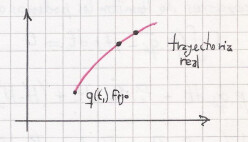
\includegraphics[scale=0.5]{images/fig_mc_ham-jac_1.jpg}

El diferencial de la integral resulta, como hemos visto en incontables ocasiones para Euler-Lagrange, en
\[
	\delta S = \left. \dpar{ \Lag }{ q_i } \delta q_i \right|_{t_1}^{t_2} + 
	\int_{t_1}^{t_2} \left[ \dpar{ \Lag }{ q_i } - \dtot{}{t}\Dpar{\Lag}{\dot{q}_i} \right] \delta q_i \: dt. 
\]

Luego, $ \delta S = p_i \delta q_i  $ y entonces $ p_i = dS / dq_i $. Como $\Lag = dS / dt $
\[
	\dtot{S}{t} = \dpar{S}{t} + \dpar{S}{q_i} \dot{q}_i \qquad \Lag = \dpar{S}{t} + p_i \dot{q}_i
\]
A partir de esta última, el diferencial $d\Lag$ es
\[
	d\Lag = \dot{p}_i dq_i + p_i d\dot{q}_i + \dpar{\Lag}{t}
\]
\[
	d\Lag = \dot{p}_i dq_i + p_i d\dot{q}_i + d( p_i \dot{q}_i ) + \dpar{\Lag}{t},
\]
de manera que 
\[
	d( \Lag - p_i \dot{q}_i ) = p_i dq_i - q_i dp_i
\]
lo que nos lleva a las ecuaciones de Hamilton
\[
	\dot{p}_i = - \dpar{H}{q_i} \qquad \dot{q}_i = \dpar{H}{p_i} \qquad \dpar{H}{t} = - \dpar{\Lag}{t} 
\]

Entonces
\[
	S = \int ( p_i \dot{q}_i - H ) \: dt,
\]
y pidiendo $\delta S=0$ se tiene 
\[
	\delta S = \int_{t_1}^{t_2}  \: \left[ \dtot{}{t}( p_i \delta q_i ) - \dot{p}_i \delta q_i + \dot{q}_i \delta p_i 
	- \dtot{H}{p_i} \delta q_i - \dpar{H}{p_i} \delta p_i \right] \: dt
\]
o bien 
\[
	\left. p_i \delta q_i \right|_{t_1}^{t_2} - \int dt 
	\left[ \left( \dot{p}_i + \dpar{H}{q_i} \right) \delta q_i + ( \dtot{H}{p_i} - \dot{q}_i ) \delta p_i \right]
\]

Entonces las ecuaciones de Hamilton las podemos obtener con 
\[
	\delta \int ( p_i \dot{q}_i - H ) dt = 0 \qquad \delta \int ( P_i \dot{Q}_i - H' ) dt = 0
\]
y
\[
	dF_1 = p_i \dot{q}_i dt - P_i \dot{Q}_i dt + (H'-H)dt
\]
\[
	dF( qq_i, Q_i, t ) = P_i dq_i - P_i dQ_i + (H'- H)dt
\]
y de la {\it lectura} de 
\[
	dF_1 =
\]
se identifican 
\[
	\dtot{F_1}{q_i} = p_i \qquad \qquad \dtot{F_1}{P_i} = -P_i.
\]

De modo ídem se tiene 
\[
	d(F_1 + P_iQ_i) = P_i dq_i + Q_i dP_i + (H'-H)dt
\]
($F_2(q_i,P_i,t)$) lo que lleva a 
\[
	\dtot{F_2}{q_i} = p_i \qquad \qquad \dtot{F_2}{P_i} = Q_i \qquad \qquad \dtot{F_2}{t} = H'- H.
\]

Entonces
\[
	\dpar{S}{t} + H(q_i,\dpar{S}{q_i},t) = 0
\]
pero la derivada parcial en el argumento es $p_i$. La transformación $(q_i,p_i) \to (Q_i,P_i) = (\beta_i,\alpha_i)$ 
permite la escritura
\[
	\dpar{S}{t} + H(q_i,\alpha_i,t) = 0,
\]
y $S = S'(\alpha_i) + A$ donde los $\alpha_i$ son $n$ variables (dado que $S$ aparece sólo derivada).
\[
	\dpar{S}{\alpha_i} = \beta_i \qquad H'= H + \dpar{S}{t} = 0
\]
y entonces $ \dot{\alpha}_i = 0, \dot{\beta}_i=0 $. Ahora como los momentos y las coordenadas son constantes el problema
es trivial pero la transformación es muy jodida.
\[
	\dpar{S}{t} + H(q_i,\dpar{S}{q_i}) = 0 \qquad \qquad S = S(q_i,t)
\]
en este caso $ \dtot{S}{t} = -E $ y se tiene 
\[
	S = W\left( q_i,\dpar{S}{q_i} \right) - E t.
\]



% =================================================================================================
\section{Potencial electromagnético}
% =================================================================================================

Arranquemos por los momentos canónicamente conjugados
\[
	\dpar{\Lag}{\dot{q}_i} = p_i \quad \textrm{pero} \; si V \neq V(q) \longrightarrow \dpar{T}{\dot{q}_i} = p_i
\]
entonces
\[
	U(q,\dot{q}) =  e \phi - e/c \vb{A}\cdot\vb{V} \longrightarrow \Lag = T - e \phi + e/c  \vb{A}\cdot\vb{V}
\]
\[
	p_x = \dpar{T}{\dot{x}} - \dpar{U}{\dot{x}} = m V_x - (e/c) A_x.
\]

Hacemos un cambio de gauge, en un potencial generalizado
\[
	U =  e \Phi(\vb{x},t) - (q/c) \vb{A}(\vb{x},t)\cdot\vb{V}(t)
\]
y el cambio de gauge es
\[
	\vb{A}' = \vb{A} + \nabla f,
\]
que no altera las ecuaciones de movimiento.


\begin{ejemplo}{\bf Problema de parcial}

El problema cuya geometría se ilustra a continuación. Se consideran $m_1 = m_2 = m$, $m_3 = M$ y  $k$ {\it slinkies}.

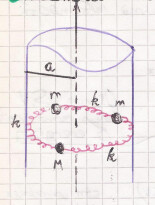
\includegraphics[scale=0.5]{images/fig_mc_problema_parcial_osc_0.jpg}
 
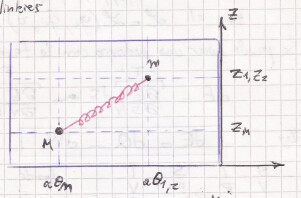
\includegraphics[scale=0.5]{images/fig_mc_problema_parcial_osc_1.jpg}

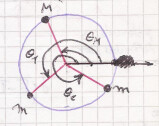
\includegraphics[scale=0.5]{images/fig_mc_problema_parcial_osc_2.jpg}

Es claramente un problema de seis grados de libertad, $\theta_M, \theta_1, \theta_2, Z_M, Z_1, Z_2$ 

Podemos escribir la energía cinética y el potencial como 
\[
	T = \frac{1}{2} M a^2 \dot{\theta}_M^2 + \frac{1}{2} M a^2 (\dot{\theta}_1^2 + \dot{\theta}_2^2 ) +
	\frac{1}{2} M \dot{Z}_M^2 + \frac{1}{2} m ( \dot{Z}_1^2 + \dot{Z}_2^2 )
\]
\[
	V = \frac{1}{2} \left[ a^2 ( \theta_2 - \theta_M ) + ( Z_2 - Z_M )^2 \right] +
	\frac{1}{2} \left[  a^2 ( \theta_1 - \theta_2 ) + ( Z_1 - Z_2 )^2 \right] +
	\frac{1}{2} \left[ a^2 ( \theta_1 - \theta_M ) + ( Z_1- Z_M )^2 \right] 
\]
\[
	\Lag = T - V
\]
Como ya está en forma cuadrática no es necesario aproximar. Si tenemos expresiones lineales habría que desarrollar
a orden dos, por ejemplo $ \cos \theta \sim 1 - \theta^2/2 $ y me quedo con los términos cuadráticos.

Definimos coordenadas referidas al equilibrio. Nos paramos en el equilibrio y oscilamos en torno a él.
\[
 	\eta_1 = ( \theta_M - \theta_{\mbox{eq}} ) 
 	\qquad 
 	\eta_2 = ( \theta_M - \theta_{ 1 \mbox{eq} } )a 
 	\qquad 
 	\eta_3 = ( \theta_2 - \theta_{ 2 \mbox{eq} } )a
\]
\[
	\eta_4 = Z_M - Z_{M\mbox{eq}} \qquad \eta_5 = Z_1 - Z_{1\mbox{eq}} \qquad \eta_6 = Z_2 - Z_{2\mbox{eq}}
\]
con sus correspondientes velocidades
\[
	\dot{\eta}_1 = a \dot{\theta}_M \qquad \dot{\eta}_2 = a \dot{\theta}_1 \qquad \dot{\eta}_3 = a \dot{\theta}_2
\]
\[
	\dot{\eta}_4 = \dot{Z}_M \qquad \dot{\eta}_5 = \dot{Z}_1 \qquad \dot{\eta}_6 = \dot{Z}_2
\]

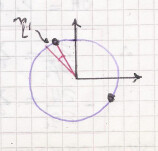
\includegraphics[scale=0.5]{images/fig_mc_problema_parcial_osc_3.jpg}

El lagrangiano será 
\begin{multline*}
	\Lag  =  \frac{1}{2} M \dot{\eta}_1^2 + \frac{1}{2}\dot{\eta}_4^2 + \frac{1}{2} m (\dot{\eta}_2^2 + \dot{\eta}_3^2 + \dot{\eta}_5^2 + \dot{\eta}_6^2 ) \\
	- \frac{k}{2}\left[ (\eta_1 - \eta_2 )^2 + (\eta_5 - \eta_4 )^2 + (\eta_1 - \eta_3 )^2 + (\eta_6 - \eta_4 )^2 + (\eta_2 - \eta_3 )^2 + (\eta_5 - \eta_6 )^2 \right]
\end{multline*}


Habria que identificar los coeficientes para armar $T,V$ en 
\[
	\Lag = \frac{1}{2} \dot{\bar{eta}}^\dagger \mathbb{T} \dot{\bar{eta}} 
	- \frac{1}{2} \bar{eta}^\dagger \mathbb{V} \bar{eta}
\]

Como ejemplo, desarrollemos algún término
\[
	k(\eta_1 - \eta_2)^2 = k \eta_1 \eta_2 - 2k \eta_1 \eta_2 + k \eta_2 \eta_2 =
	k \eta_1 \eta_2 - k \eta_1 \eta_2 -  k \eta_1 \eta_2 + k \eta_2 \eta_2
\]

Las matrices resultan 
\[
	V = \begin{pmatrix}
	     2 k & -k & -k & 0 & 0 & 0 \\
	     -k & 2k & -k & 0 & 0 & 0 \\
	     -k & -k & 2k & 0 & 0 & 0 \\
	     0 & 0 & 0 & 2k & -k & -k \\
	     0 & 0 & 0 & -k & 2k & -k \\
	     0 & 0 & 0 & -k & -k & 2k
	    \end{pmatrix}
\]
\[
	T = \begin{pmatrix}
	     M & 0 & 0 & 0 & 0 & 0 \\
	     0 & m & 0 & 0 & 0 & 0 \\
	     0 & 0 & m & 0 & 0 & 0 \\
	     0 & 0 & 0 & M & 0 & 0 \\
	     0 & 0 & 0 & 0 & m & 0 \\
	     0 & 0 & 0 & 0 & 0 & m 
	    \end{pmatrix}
\]
y como se ve ambas resultan en bloques de Jordan y son cada bloque igual. El a incluido en la coordenada hace que se
obtenga esa forma simétrica.
En
\[
	\mbox{det}( \mathbb{V} - \omega^2 \mathbb{T} )
\]
se reduce a calcular el determinante de la submatriz de 3 $\times$ 3,
\[
	\begin{bmatrix}
	2 k - \omega^2 M & -k & -k \\
	-k & 2 k - \omega^2 m & -k \\
	-k & -k & 2 k - \omega^2 m 
	\end{bmatrix}
\]
que resulta en la ecuación 
\[
	\omega^2 \left( \omega^4 - \omega^2 \left[  \frac{2k}{M} + \frac{2k}{M} \right] +
	\left[ \frac{6k^2}{mM} + \frac{3k^2}{m^2} \right] \right) = 0,
\]
que da 
\[
	\omega_1^2 = 0 \qquad \qquad \omega_2^2 = \frac{2k}{M} + \frac{k}{m} \qquad \qquad \omega_3^2 = \frac{3k}{m} 
\]

Para $\omega^2 = 0$ la ecuación $ (V - \omega^2 T )A^1 = 0 $ se verifica para 
\[
	A^1 = \alpha \begin{pmatrix} 1 \\ 1 \\ 1 \end{pmatrix}
\]
cuya normalización se ajusta con $ {A^\dagger}^1 T A^1 = 1$ o bien 
\[
	\alpha^2 \begin{pmatrix} 1 & 1 & 1 \end{pmatrix}
	\begin{pmatrix}
	 M & 0 & 0 \\
	 0 & m & 0 \\
	 0 & 0 & m
	\end{pmatrix}
	\begin{pmatrix} 1 \\ 1 \\ 1 \end{pmatrix} = 1,
\]
siendo el valor de $\alpha$ dado por 
\[
	\alpha^2 = \frac{1}{2m+M} \qquad \alpha = \frac{1}{ \sqrt{2m+M} }.
\]

Los autovectores son 
\[
	A^1 = \frac{1}{\sqrt{M + 2m}} \begin{pmatrix} 1 \\ 1 \\ 1 \end{pmatrix} \qquad 
	A^2 = \frac{1}{\sqrt{4m^2/M + 2m}} \begin{pmatrix} -2m/M \\ 1 \\ 1 \end{pmatrix} \qquad 
	A^3 = \frac{1}{\sqrt{ 2m }} \begin{pmatrix} 0 \\ 1 \\ -1 \end{pmatrix} \qquad 
\]
 
Los movimientos están dados por

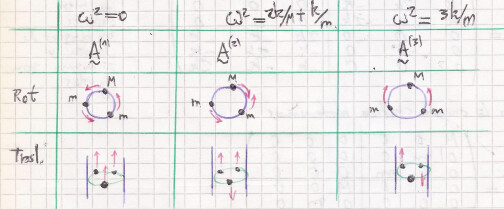
\includegraphics[scale=0.5]{images/fig_mc_problema_parcial_osc_4.jpg}
 
Ahora hay que completar hasta la sexta dimensión
\[
	\bar{\eta}_1 = \frac{1}{\sqrt{2m+M}} \begin{pmatrix} 1 \\ 1 \\ 1 \\ 0 \\ 0 \\ 0
	                                     \end{pmatrix} \qquad \qquad
	\bar{\eta}_3 = \frac{1}{\sqrt{2m}} \begin{pmatrix} 0 \\ 1 \\ -1 \\ 0 \\ 0 \\ 0
	                                     \end{pmatrix} \qquad \qquad
	\bar{\eta}_5 = \frac{1}{\sqrt{2m + 4m^2/M}} \begin{pmatrix} 0 \\ 0 \\ 0 \\ -2m/M0 \\ 1 \\ 1
	                                     \end{pmatrix}
\]
\[
	\bar{\eta}_2 = \frac{1}{\sqrt{2m+ 4m^2/M}} \begin{pmatrix} -2m/M \\ 1 \\ 1 \\ 0 \\ 0 \\ 0 
						\end{pmatrix} \qquad \qquad
	\bar{\eta}_4 = \frac{1}{\sqrt{M + 2m}} \begin{pmatrix} 0 \\ 0 \\ 0 \\ 1 \\ 1 \\ 1
	                                     \end{pmatrix} \qquad \qquad
	\bar{\eta}_6 = \frac{1}{\sqrt{2m}} \begin{pmatrix} 0 \\ 0 \\ 0 \\ 0 \\ 1 \\ -1
	                                     \end{pmatrix}
\] 
 
Luego, para desacoplar la solución habría que plantear la matriz
\[
	\mathbb{B} = [ \eta^\dagger_1 ... \eta_i^\dagger ]
\]
 
\end{ejemplo}

\begin{ejemplo}{\bf Problema 12}

El setup se ilustra en la figura siguiente.

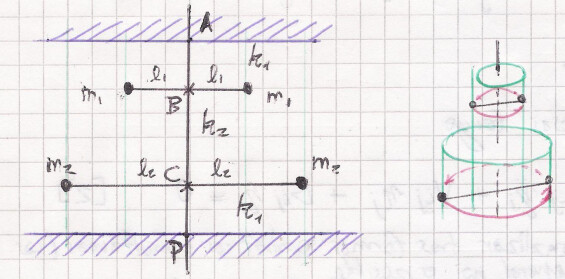
\includegraphics[scale=0.5]{images/fig_mc_problema_12.jpg}

El torque 
\[
	\tau = - k \theta
\]
lo suponemos un potencial $ V = 1/2 k \theta^2 $, donde $k$ tiene unidades de energía.
Las barras solo rotan de manera que 
\[
	T_1 = \frac{1}{2} ( m_1 \ell_1^2 \dot{\theta}_1^2  ) + \frac{1}{2}( m_1 \ell_1^2 \dot{\theta}^2_1 )
\]
donde estamos pensando como dos partículas. En cambio, pensándolo como una barra con momento de inercia es
\[
	T = \frac{1}{2} I \Omega^2
\]

Entonces,
\[
	T = T_1 + T_2 = \frac{1}{2} ( 2 m_1 \ell_1^2 \dot{\theta}_1^2  ) + \frac{1}{2}( 2 m_2 \ell_2^2 \dot{\theta}^2_2 )
\]
\[
	V_1 = \frac{1}{2} k_1 \theta^2_1 \qquad 
	V_{12} = \frac{1}{2} k_2 ( \theta_2 - \theta_1 )^2  \qquad 
	V_2 = \frac{1}{2} k_1 \theta^2_2 
\]

Definiendo $\eta_i = \theta_i - \theta_{\mbox{eq}}$ que implican $\dot{\eta}_i = \dot{\theta}_i $ $(i=1,2)$ se puede escribir el lagrangiano como 
\[
	\Lag = \ell_1^2 m_1 \dot{\eta}_1^2 + \ell_2^2 m_2 \dot{\eta}_2^2 - \frac{1}{2} k_1 \eta_1^2 - \frac{1}{2} k_2 \eta_2^2 - \frac{1}{2} k_2 (\eta_2 - \eta_1)^2
\]
de manera que 
\[
	\mathbb{T} = \begin{pmatrix}
	 2 \ell^2_1 m_1 & 0 \\
	 0 & 2 \ell^2_2 m_2 
	\end{pmatrix}
	\qquad 
	\mathbb{V} = \begin{pmatrix}
	 k_1 + k_2 & - k_2 \\
	 -k_2  & k_1 + k_ 2 
	\end{pmatrix}
\]

Faltaría entonces
\[
	\mbox{det} \{ \mathbb{V} - \omega^2 \mathbb{T} \} = 0
\]
y los autovectores $A^1, A^2$.


\end{ejemplo}

\begin{ejemplo}{\bf Problema 8}

Un problema de pequeñas oscilaciones.

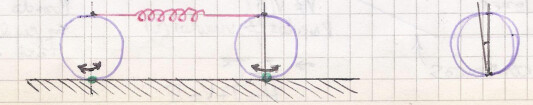
\includegraphics[scale=0.5]{images/fig_mc_problema_8.jpg} 

En este ejemplo hay que suponer que el lagrangiano es ya de entrada de pequeñas oscilaciones.

\end{ejemplo}

\begin{ejemplo}{\bf Problema 1 P96}

El lagrangiano para el {\it setup} es 
\[
	\Lag = \frac 1 2 m ( \dot{x}^2 + \dot{y}^2 + \dot{z}^2 ) - \frac{k_x}{2} x^2 - \frac{k_y}{2} y^2 - \frac{k_z}{2} z^2,
\]
donde los momentos son 
\[
	p_i = \dpar{\Lag}{\dot{x}_i} = m\dot{x}_i,
\]
para cada una de las coordenadas. El hamiltoniano es $h = \sum_i p_i \dot{q}_i - \Lag$, que explícitamente
\[
	h = \frac{p_x^2}{2m} + \frac{p_y^2}{2m} + \frac{p_z^2}{2m} + \frac{k_x}{2} x^2 + \frac{k_y}{2} y^2 + \frac{k_z}{2} z^2
\]
de donde leemos
\[
	\dpar{H}{x} = k_x x = - \dot{p}_x \qquad \dpar{H}{p_x} = \frac{p_x}{m} = \dot{x},
\]
que conduce, derivando una vez más, a $ \ddot{x} = \dot{p}_x / m $ y $ \ddot{x} = - k_x / m $, que es la ecuación del oscilador
armónico en $x$.
 
El diagrama de fases es algo como lo que muestra la figura siguiente
 
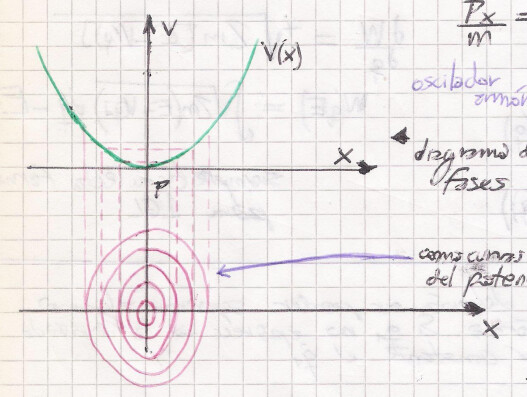
\includegraphics[scale=0.35]{images/fig_mc_problema_1_p96.jpg} 

donde bajo el primer gráfico aparecen las curvas de nivel del potencial.

Para fuerza central resulta $U(r)$ en esféricas y el lagrangiano es
\[
	\Lag =
\]
Calculando el hamiltoniano según la definición resulta, después de algo de álgebra, en
\[
	\Ham = \frac{p_r^2}{2m} + \frac{1}{2mr^2} \left( p_\theta^2 + \frac{p_\vp^2}{\sin^2\theta}\right) + U(r) .
\]
El hamiltoniano es constantes puesto que el lagrangiano no depende del tiempo y $p_\vp$, por la ciclicidad de $\vp$
es constante.

Si espedificamos como potencial el de Kepler, vemos que es separable en $\theta, r$ puesto que se tiene 
\[
	f(\theta,\vp) = g(r)
\]
de modo que cada una de estas funciones es una constante.

La conservación del momento angular en términos del hamiltoniano resulta en
\[
	\dtot{}{t} \left( p_\theta^2 + \frac{p_\vp^2}{\sin^2\theta}\right) = 2 p_\theta \dot{p}_\theta +
	\frac{ 2 p_\vp^2 \dot{p}_\vp^2}{\sin^2\theta} - \frac{2\cos\theta\dot{\theta}p_\vp^2}{\sin^3\theta}
\]
y entonces
\[
	\dot{p}_\theta = -\dpar{\Ham}{\theta} \left( \frac{-1}{2mr^2} \frac{-4p_\vp^2 \sin^2\theta \cos\theta}{\sin^2\theta} \right),
\]
y eso lleva a 
\[
	 \left( p_\theta^2 + \frac{p_\vp^2}{\sin^2\theta}\right) = cte
\]

EL hamiltoniano tiene un potencial efectivo dado por los dos últimos términos de la derecha,
\[
	\Ham = \frac{p_r^2}{2m} + \frac{1}{2mr^2} L^2 + U(r)
\]

El diagrama de fases aparece aquí abajo.

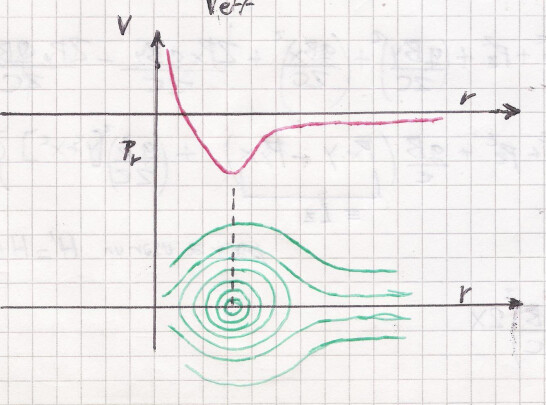
\includegraphics[scale=0.35]{images/fig_mc_problema_1_p96_2.jpg} 
 
\end{ejemplo}


\begin{ejemplo}{\bf Problema 8 P97}

Consideramos un potencial generalizado
\[
	U = q \vp - \frac q c \vb{v}\cdot\vb{A},
\]
donde $\vb{A} = 1/2 \pv{B}{x}$ y asimismo $\pv{\nabla}{A}=\vb{B}$ siendo el lagrangiano,
\[
	\Lag = \frac 1 2 m ( \dot{x}^2 + \dot{y}^2 + \dot{z}^2 ) + \frac{q}{c} \vb{v}\cdot\vb{A}
\]

Si el campo está en el eje $z$, es decir $\vb{B}=(0,0,B)$ se tiene $\vb{A} = 1 /2 ( -B y \hat{x} + B x \hat{y} )$, lo
cual conduce a 
\[
	\Lag = \frac 1 2 m ( \dot{x}^2 + \dot{y}^2 + \dot{z}^2 ) + \frac{q}{c} \frac{B}{2} ( - \dot{x} y + \dot{y} x )
\]
y los momentos son
\[
	P_x = m \dot{x} - \frac{qB}{2c}y \qquad
	P_y = m \dot{y} + \frac{qB}{2c}x \qquad 
	P_z = m \dot{z}  
\]
de manera que $z$ es cíclica. Luego, calculando el hamiltoniano a través de la definición es 
\[
	\Ham = \frac{1}{2} m ( \dot{x}^2 + \dot{y}^2 + \dot{z}^2 ),
\]
o bien (usando las equivalencias anteriores)
\[
	\Ham = \frac{1}{2m} \left[ p_x^2 + p_y^2 + p_z^2 + \frac{qB}{c}\left( p_x y - p_y x \right) +
	\Frac{qB}{2c}^2( x^2 + y^2 ) \right], 
\]
y el paréntesis dentro del corchete es el $L_z$.
Paso a usar un hamiltoniano $\Ham' = \Ham + cte.$
\[
	\dot{x} = \dpar{\Ham'}{p_x} = \frac{p_x}{m} \qquad \dot{p_x} = -\dpar{\Ham'}{x} = \frac{1}{2m}\Frac{qB}{2c}^2 2x
\]

Obtenemos para la ecuación de Newton,
\[
	\ddot{x} - \frac{q^2 B^2}{4 c^2 m^2} x = 0
\]
mientras que para la coordenada $y$ obtenemos una ecuación similar. Entonces
\[
	\ddot{x} + \omega^2 x = 0 \qquad \ddot{y} + \omega^2 y = 0
\]
con $\omega = q B / ( 2 c m )$. Luego
\[
	x = \frac{1}{\sqrt{ }}( \sqrt{ 2p } + ) \qquad y = \frac{1}{\sqrt{ }}( \sqrt{ 2p } + )
\]
y sus correspondienes momentos,
\[
	p_x = \frac{\sqrt{ }}{2} () \qquad p_y = \frac{\sqrt{ }}{2} ()
\]
 
Deberíamos probar que es una transformación canónica chequeando que se verifican
\[
	[ x, p_x ], [ y, p_y ] = cte. \qquad [ x, y ] = [ p_x, p_y ] = 0
\]
\[
	[ x, p_x ] = sum_i \dpar{x}{q_i} \dpar{p_x}{p_i} - \dpar{p_x}{q_i} \dpar{x}{p_i}
\]
y las derivadas
\[
	\dpar{x}{q_1} = \frac{1}{\sqrt{m\omega}} ( \sqrt{ 2p_1} \cos q_1 ) \qquad \dpar{x}{q_2} = 0
\]
\[
	\dpar{x}{p_1} = \frac{1}{\sqrt{2 m p_1}} ( \sin q_1 ) \qquad \dpar{x}{p_2} = \frac{1}{\sqrt{m\omega}}
\]
\[
	\dpar{p_x}{q_1} = -\frac{\sqrt{2 m p_1}}{2} ( \sin q_1 ) \qquad \dpar{p_x}{q_2} = -\frac{\sqrt{m \omega}}{2} \qquad \dpar{p_x}{p_2} = 0
\] 
\[
	\dpar{p_x}{p_1} = \frac{\sqrt{ }}{\sqrt{2p_1}}
\]
\[
	[ x, p_x ] = \frac{1}{ \sqrt{ m \omega} } \sqrt{ 2 p_1 } \cos^2 q_1 + \left( \frac{\sqrt{2 m p_1}}{2} \sin^2 q_1 \right) + \frac{1}{2}
\]

El hamiltoniano luce
\[
	\Ham = \frac{1}{2m} \left( p_x^2 + p_y^2 + \frac{m^2\omega^2}{4}[ x^2 + y^2 ] \right)
\]
\[
	\Ham = \frac{\omega}{2} p_1 + \frac{\omega}{4} p_2^2 + \frac{\omega}{4} q_2^2,
\]
y se ve que $q_1$ resultó cíclica. Luego $p_1$ es una constante y 
\[
	\dot{p}_2 = \dpar{\Ham}{q_2} = \frac{\omega}{2} q_2.
\]
Resolviendo se llega a 
\[
	\ddot{q}_2 + \omega^2 q_2 = 0,
\]
de manera que $q_2$ tiene comportamiento oscilatorio. Pero
\[
	\dot{q}_1 = -\dpar{\Ham}{p_1} = \frac{\omega}{2} \qquad q_1 = - \frac{\omega}{2} t.
\]
\end{ejemplo}

\begin{ejemplo}{\bf Hamilton Jacobi para fuerza central}

\[
	\Ham = \frac{1}{2m} p_r^2 + \frac{1}{2mr^2}p_\vp^2 + V(r), \qquad S = S' - Et
\]
entonces se puede escribir
\[
	E  - \left[ \frac{1}{2m}\Dpar{S}{r}^2 + V(r) \right] = \frac{1}{2m}\Dpar{S}{\vp}^2.
\]

Para esféricas necesitaré:
\[
	V = V(r) + \frac{b(\theta)}{r^2} + \frac{c(\vp)}{r^2 \sin^2\theta}
\]

Si reemplazo en el hamiltoniano a la forma separable
\[
	W(r, \theta, \vp) = W'(r, \theta) + S_\vp(\vp),
\]
de modo que 
\[
	\Dpar{S}{\vp}^2 + C(\vp) = \alpha \vp
\]
que ya se integra directamente. Luego en forma ídem es
\[
	W'(r, \theta) = S_r( r ) + S_\theta(\theta).
\]
\end{ejemplo}

\begin{ejemplo}{\bf Otro ejemplo de potencial}

\[
	V = \frac{\alpha}{r} - F(z) \qquad \qquad ( r \text{ esféricos}, z \text{ cilíndricas })
\]
donde $(\xi, \eta, \vp)$ coordenadas parabólicas. Verifican
\[
	\frac{ a(\xi) + b(\eta) }{\xi + \eta}
\]
\[
	z = \frac 1 2 ( \xi - \eta ), \quad \rho =  \sqrt{\xi \eta}, \quad \vp \in \{ 0, 2\pi \}, 0 < \xi, \eta < \infty 
\] 
\[
	r = \sqrt{ \rho^2 + z^2 } = \sqrt{ \frac{1}{4} ( \xi - \eta )^2 + \xi \eta },
\]
de modo que $r = 1/2 (\xi + \eta)$. Consideremos
\[
	\Lag  = \frac{1}{2m} ( \dot{\rho}^2 + \rho^2 \dot{\vp}^2 + \dot{z}^2 ) - V(\rho,\vp,z)
\]
que lleva a 
\[
	\dot{\rho}^2 + \dot{z}^2 = \frac{1}{4} ( \xi + \eta )\left( \frac{\dot{\xi}^2}{\xi} + \frac{\dot{\eta}^2}{\eta} \right)
\]

El lagrangiano es
\[
	\Lag = \frac{1}{8} m (\xi + \eta) \left( \frac{\dot{\xi}^2}{\xi} + \frac{\dot{\eta}^2}{\eta} \right) +
	\frac{m}{2}\xi\eta\dot{\vp}^2 - V(\xi,\eta,\vp)
\]
y los momentos 
\[
	p_\xi = \dpar{\Lag}{\dot{\xi}} = \frac{m}{4} (\xi + \eta) \frac{\dot{\xi}}{\xi} \qquad 
	p_\eta = \frac{m}{4} (\xi + \eta) \frac{\dot{\eta}}{\eta}, \qquad
	p_\vp = m \xi \eta \dot{ \vp }
\]
mientras que el hamiltoniano es
\[
	\Ham = \frac{2}{m} \Frac{ \xi p_\xi^2 + \eta p_\eta^2 }{ \xi + \eta } + \frac{ p_\vp^2 }{ 2 m \xi \eta } + 
	\frac{ a(\xi) + b(\eta) }{ \xi + \eta }
\]

Ahora vemos el potencial $V(r,z)$ que es 
\[
	V = \frac{1}{r} ( \alpha - Fr ) = \frac{1}{r} ( \alpha - \frac{1}{4} F ( \xi^2 - \eta^2 ) )
\]
\[
	V = \frac{( \alpha - F \xi^2 / 2 ) + ( \alpha + F \eta^2 / 2 )}{\xi + \eta}
\]
 
Reemplazando en el hamiltoniano se tiene 
\[
	S = W(\xi,\eta,\vp) - Et = W(\xi,\eta) + p_\vp \vp - Et
\]
donde
\[
	E(\xi + \eta) = 2 \xi \Dpar{W}{\xi}^2 + 2 \eta \Dpar{W}{\eta}^2 + \frac{(\xi + \eta)p_\vp}{2 m \xi \eta} + a(\xi) + b(\eta)
\]
o bien 
\[
	E\xi - 2 \xi \Dpar{W}{\xi}^2 + E\xi - \frac{p_\vp}{2 m \xi} - a(\xi) =  2 \eta \Dpar{W}{\eta}^2 + E\xi - \frac{p_\vp}{2 m \eta} + b(\eta) - E\eta  
\]
y como $ W(\xi,\eta) = W_\xi(\xi) + W_eta(\eta) $ se tiene 
\[
	\beta =  2 \xi \Dpar{W_\xi}{\xi}^2 + \frac{p_\vp}{2 m \xi} + a(\xi) -E\xi
\]
\[
	W(\xi) = \int \; \sqrt{ \frac{1}{2\xi} \left( \beta + E\xi - \frac{p_\vp}{2 m \xi} - a(\xi) \right)} d\xi,
\]
o bien
\[
	S = W_\xi(\xi) + W_\eta(\eta) + p_\vp \vp - Et
\]

\end{ejemplo}


\begin{ejemplo}{Problema interesante (reacomodar o desaparecer)}

Este sistema tiene los mismos modos normales que si no estuvieran estos nuevos resortes conectados

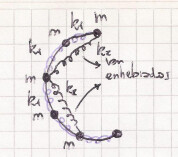
\includegraphics[scale=0.35]{images/fig_mc_problema_interesante.jpg}

La matriz con resortes entre vecinos es
\[
	\begin{pmatrix}
	2 k_1 & - k_1 & 0 & 0 & ... & - k_1 \\ 
	-k_1 & 2k_1 & -k_1 & 0 & ... & - k_1 \\
	0 & - k_1 & 2k_1 & ... &  \\
	& 0 & 0 & ...& & -k_1 \\
	& & &... & 2k_1 & 0 \\
	-k_1 &  &  & -k_1 & 0 & 2k_1
	\end{pmatrix}
\]
mientras que la matriz con resortes entre terceros
\[
	\begin{pmatrix}
	2 (k_1 +k_2) & - k_1 & -k_2 & 0 & ... & - k_1 \\ 
	-k_1 & 2(k_1+k_2) & -k_1 & 0 & ... & - k_1 \\
	k_2 & - k_1 & 2(k_1+k_2) & ... &  \\
	& 0 & 0 & ...& 2k_1 &  \\
	-k_2& & &... &  & -k_1 \\
	-k_1 & -k_2 &  &  & -k_1 & 2k_1
	\end{pmatrix}
\]

Siempre tiene los mismos autovectores.
Los modos normales están dados por la geometría y las condiciones de contorno.

\end{ejemplo}

\subsection{Popurrí de cosas para reubicar}

{\bf Sobre el potencial}
Si $\vb{F}$ proviene de un potencial que depende del tiempo entonces no será conservativo el campo de fuerzas.
No vale lo mismo la integral $\int F(x,t) dx$ por diferentes caminos (dependerá del tiempo que tarde en cada
camino).

{\bf sobre generatrices}
\[
	F_2 = F_1 + \sum  Q_i P_i,
\]
con
\[
	\begin{cases}
	Q_i = Q_i( q_i, P_i ) \\
	P_i = P_i( q_i )
	\end{cases}
\]
pero tienen que estar escritas $Q_i, P_i$ en términos de las variables de $F_2$

{\bf Ángulo-acción}

Todas los grados de libertad separables (de lo contrario no puedo definir una de las acciones).

{\bf Observación}

Se puede transformar entre $n$ grados de libertad dependiendo del tiempo a $n+1$ grados de 
libertad conservativos.

{\bf Bundle de Hamilton-Jacobi}

Resolviendo Hamilton-Jacobi llego a
\[
	K = H(q_i,) - E = 0
\]
y si $t$ es separable paso al problema $ H(q_i,) = E $.
\[
	\dpar{W}{q_i} = p_i \qquad \qquad \dpar{W}{P_i} = Q_i
\]
con 
\[
	\theta_i = \omega_i(J_1,...,J_n) t + \theta_{i0}
\]
\[
	\dpar{E}{J_i}(J_1,...,J_n) = \dot{\theta}_i = \omega_i (J_1,...,J_n)
\]

El problema general tiene como solución $J_i$ constante $\theta$ lineal.
El asunto es pasar a la solución que sirve 
\[
	\begin{cases}
	q_1(t), ..., q_n(t) \\
	p_1(t), ..., p_n(t)
	\end{cases}
\]
usando las condiciones iniciales y la generatriz $S$.

La derivada
\[
	\dpar{W}{q_i} = p_i(q_1,... , q_n,J_1,...,J_n)
\]
hay que expresarla en función de los nuevos momentos $J_i$ (no de las constantes de separación $\alpha_i$) pero
en realidad el problema es totalmente separable, entonces
\[
	\dpar{W}{q_i} = p_i(q_i,J_1,..,J_n)
\]
para ángulo-acción los $P_i$ no son las constantes de separación.
\[
	W = W(q_i,P_i) \qquad W = W(q_i,J_i)
\]

Energía en función de los momentos
\[
	W = \int \sqrt{ 2 m ( E[J] - V[q] ) } dq, 
\]
entonces $W = W( J, q )$. Si tenemos varios grados de libertad tendremos varias integrales
\[
	\dpar{W}{J_i} = \theta_i(q_i,J_n) = \omega_i t + \theta_{i0}
\]

Con las condiciones iniciales me meto en:
\[
	\dpar{W}{q_i}(q_1,J_1,...,J_n) = p_i(q_1,... , q_n,J_1,...,J_n)
\]
con los $p_{i0}$ y los $q_{i0}$ obtengo los $J_1, ..., J_n$ constantes $n$ ecuaciones $p_{i0} = p_i (q_1,J_1,...,J_n)$
\[
	\dot{\theta}_i = \omega_i (J_1, ..., J_n )
\]
con los $J_1, ..., J_n$ obtengo $\dot{\theta}_i$.

% \bibliographystyle{CBFT-apa-good}	% (uses file "apa-good.bst")
% \bibliography{CBFT.Referencias} % La base de datos bibliográfica


\begin{ejercicios}

\label{ej1}
\item{ \bf }
Escriba el hamiltoniano y las ecuaciones de Hamilton para
\begin{enumerate}[label=(\alph*)]
\item Un oscilador armónico tridimensional (no necesariamente isótropo). Utilizar co-
ordenadas cartesianas.
\item Una partı́cula en un potencial central U (r)
\item Un trompo simétrico con un punto fijo en el campo gravitatorio terrestre.
\end{enumerate}
En a., resuelva las ecuaciones. En b. y c., halle constantes de movimiento. Particulari-
zando en b. a U (r) = −k/r, discuta las órbitas posibles. En todos los casos construya
los diagramas de fases correspondientes.

\label{ej2}
\item{ \bf }
Escriba y resuelva las ecuaciones de Hamilton para un oscilador armónico tridimen-
sional isótropo en coordenadas cilı́ndricas y en coordenadas esféricas. Construya los
correspondientes diagramas de fases.

\label{ej3}
\item{ \bf }
Una partı́cula en un campo gravitatorio uniforme se mueve sobre la superficie de una
esfera centrada en el origen. El radio de la esfera varı́a en el tiempo: r = r(t), donde
r(t) es una función conocida. Obtenga el hamiltoniano y las ecuaciones canónicas.
Discuta la conservación de la energı́a. Es el hamiltoniano la energı́a total?.

\label{ej4}
\item{ \bf }
Considere una partı́cula moviéndose en un plano bajo la influencia del potencial ge-
neralizado V = 1r (1 + ṙ2 ), donde r es la distancia al origen. Encuentre los momentos
generalizados pr y pθ y H. Obtenga las ecuaciones canónicas y muestre que el impulso
angular se conserva. Se conserva H?. Es H = E?. Reduzca el problema para r a una
ecuación diferencial de primer orden.

\label{ej5}
\item{ \bf }
Considere un oscilador armónico unidimensional:
\begin{enumerate}[label=(\alph*)]
\item Halle su hamiltoniano y las correspondientes ecuaciones de Hamilton, construya
los diagramas de fases, halle puntos de equilibrio y discuta su estabilidad, discuta
la existencia de movimientos de libración y rotación.
\item Halle la trasformación canónica de función generatriz: F1 (Q, q) = λq 2 cot Q
eligiendo λ para que el nuevo hamiltoniano sea K(Q, P ) = ωP (ω: pulsación del
oscilador).
\item Muestre que (Q, P ) son variables de ángulo–acción. Halle el área encerrada por
las curvas de E (energı́a) constante en el espacio de fases, y muestre que la curva
que corresponde a un P dado encierra un área 2πP .
\item Halle la función generatriz de tipo F2 (P, q) que genera la misma transformación
canónica (q, p) → (Q, P ). Qué relación hay entre F1 y F2 ?.
\end{enumerate}

\label{ej6}
\item{ \bf }
Considere un péndulo fı́sico constituı́do por una barra de longitud l, que puede moverse
en un plano vertical, con uno de sus extremos fijo (la barra gira libremente a su
alrededor). El momento de inercia de la barra respecto al punto fijo es I. Hay gravedad.
\begin{enumerate}[label=(\alph*)]
\item Muestre que el hamiltoniano del sistema es H = 21 I(p2ψ −2α2 cos ψ) donde ψ es el
ángulo de la barra con la vertical, pψ su momento conjugado y α una constante
a determinar.
\item Construya el correspondiente diagrama de fases; halle puntos de equilibrio y
discuta su estabilidad; construya la curva separatriz correspondiente (halle su
ecuación). Determine los movimientos de libración y rotación posibles y halle su
perı́odo.
\item Muestre que el área encerrada por la separatriz es 16α. Deduzca que el máximo
valor de la variable de acción para el movimiento de libración es 8α/π.
\end{enumerate}

\label{ej7}
\item{ \bf }
Considere los siguientes puntos:
\begin{enumerate}[label=(\alph*)]
\item Demuestre que df dt = [f, H] + ∂t . Qué obtiene para f = qi ó f = pi ?. Si
f no depende explı́citamente del tiempo, muestre que la condición necesaria y
suficiente para que f sea constante de movimiento es que [f, H] = 0.
\item Muestre que si una coordenada qi es cı́clica, la transformación canónica de función
generatriz G = pi es la transformación de simetrı́a asociada al carácter cı́clico de
qi . Observe que si f = cte. de movimiento, la transformación canónica infinite-
simal de generatriz G = f deja invariante al Hamiltoniano. Qué relación tiene
esto con el teorema de Noether?.
\end{enumerate}

\label{ej8}
\item{ \bf }
Escriba y resuelva las ecuaciones de Hamilton para una partı́cula cargada en un campo
magnético uniforme y constante B en la dirección zb.
\begin{enumerate}[label=(\alph*)]
\item Elija A = 12 B × r y resuelva el problema.
\item Demuestre que la transformación que sigue es canónica y lı́guela a una solución
alternativa de la parte a. (ω = qB/mc)
\[
	x = \frac{1}{\sqrt{m\omega}} \: \left( \sqrt{2p_1} \sin q_1 + p_2 \right)
	\qquad
	p_x = \frac{\sqrt{m\omega}}{2} \: \left( \sqrt{2p_1} \cos q_1 - q_2 \right)
\]
\[
	y = \frac{1}{\sqrt{m\omega}} \: \left( \sqrt{2p_1} \cos q_1 + q_2 \right)
	\qquad
	p_y = \frac{1}{\sqrt{m\omega}} \: \left( -\sqrt{2p_1} \sin q_1 + p_2 \right)
\]
\end{enumerate}

\label{ej9}
\item{ \bf }
Una partı́cula de masa m se mueve en el potencial:
\[
	V(x) =  \begin{cases}
			A [a^2 - (x-a)^2] \qquad \text{si } 0 \leq x \leq 2a  \; (A>0)
	        \\
	        0 \qquad \text{si } x > 2a
	        \end{cases}
\]
y choca elásticamente con la pared en x = 0. Construir el diagrama de fases corres-
pondiente, mostrando claramente las regiones de libración y movimiento no acotado.
Muestre que la variable de acción para el movimiento de libración es
\[
	J = \frac{ a^2 \sqrt{2mA} }{ 2\pi }
	\left[ \epsilon - \frac{1}{2}(1 - \epsilon^2) \: \ln \Frac{1+\epsilon}{1-\epsilon} \right]
\]
si la energı́a es E = $\epsilon^2$ a2 A (\epsilon < 1) y que el perı́odo de libración es τ = 2π dE y que si
$\epsilon$ → 1, τ → ∞.

\label{ej10}
\item{ \bf }
Una partı́cula de masa m se mueve en el potencial
\[
	V(x) =  \begin{cases}
			\frac 1 2 m \lambda^2 (x + a)^2 \qquad x \leq 0 \\
	        \\
	        \frac 1 2 m \lambda^2 (x - a)^2 \qquad x \geq 0
	        \end{cases}
\]
\begin{enumerate}[label=(\alph*)]
\item Plantee las ecuaciones de Hamilton, construya diagramas de fases, considerando
especialmente las curvas de fases próximas al origen.
\item Muestre que el espacio de fases se divide en 3 regiones invariantes, y en cada
una se definen distintas variables de ángulo–acción. Halle la variable de acción
en función de la energı́a E en cada caso.
\end{enumerate}

\label{ej11}
\item{ \bf }
Considere una partı́cula con hamiltoniano H = 2m + V (q) para cada uno de los 2 2 2 siguientes casos: V (q) = −k /q + l /2mq y V (q) = 21 mω 2 q 2 + l2 /2mq 2
\begin{enumerate}[label=(\alph*)]
\item Dibuje los diagramas de fases, escriba las ecuaciones de las curvas separatrices e
indique las regiones que corresponden a movimientos de libración y rotación.
\item Para los movimientos de libración exprese a la variable de acción como función
de la energı́a y halle la relación ψ = ψ(q, J) donde ψ es la variable de ángulo.
Cómo es la frecuencia del movimiento?.
\item Encuentre la energı́a de las trayectorias que satisfacen las relaciones J = nh̄ y
l = ph̄ (con n,p números naturales y h̄ = cte..). Discuta este punto con su
docente.
\end{enumerate}

\label{ej12}
\item{ \bf }
Una partı́cula que se mueve en una sola dimensión está sometida a un potencial dado por
\[
	V(x) = \begin{cases}
			k (x - a)^2 \qquad x > a \\
	        \\
	        \frac{V_0}{a} (a - |x|) \qquad |x| < a \\
	        \\
	        k (x + a)^2 \qquad x < -a
	        \end{cases}
\]
\begin{enumerate}[label=(\alph*)]
\item Dibuje el diagrama de fases indicando: i) en cuántas regiones queda dividido el
espacio de fases, ii) cuál es la ecuación que define a la curva separatriz, iii) cómo
son los posibles movimientos.
\item i) Calcule la variable de acción para los movimientos con E < V0 . ii) Cuánto
vale el perı́odo de dichos movimientos?. Las oscilaciones son armónicas?.
\end{enumerate}

\label{ej13}
\item{ \bf }
Escriba las variables de acción y ángulo para las rotaciones en un plano de una barra
con un punto fijo, sometida a un potencial angular V (ψ) = k|ψ|/π si −π < ψ < π
(k > 0), V (ψ) periódico [V (ψ + 2π) = V (ψ)].

\label{ej14}
\item{ \bf }
Considere el sistema de la figura: una masa m se mueve sobre un plano inclinado un
ángulo α con la horizontal y choca elásticamente con una pared en la base del plano.
Tomando como coordenada la distancia a dicho punto medida sobre el plano:
\begin{enumerate}[label=(\alph*)]
\item Construya el diagrama de fases y calcule la frecuencia del movimiento para un
dado valor de la variable de acción J.
\item Encuentre la variable de ángulo θ en función de q.
\end{enumerate}

\label{ej15}
\item{ \bf }
Resuelva los siguientes puntos
\begin{enumerate}[label=(\alph*)]
\item Escriba y resuelva las ecuaciones de Hamilton para un oscilador tridimensional
isótropo en cilı́ndricas y en esféricas. Construya los correspondientes diagramas
de fases.
\item Resuelva el problema de la partı́cula en el campo magnético uniforme B uti-
lizando como potencial vector A = Bxb y.
\end{enumerate}

\label{ej16}
\item{ \bf }
Escriba el hamiltoniano y las ecuaciones de Hamilton para:
\begin{enumerate}[label=(\alph*)]
\item un trompo simétrico que se mueve libremente (sin gravedad).
\item una máquina de Atwood, con polea sin masa y con polea de masa M y radio R.
\end{enumerate}

\label{ej17}
\item{ \bf }
Se tiene un sistema de dos masas puntuales m1 y m2 que interactúan con un potencial
V (|r1 − r2 |). Muestre que su hamiltoniano puede escribirse como H = Hcm + Hrel
\[
	H_{cm} =
	\qquad
	H_{rel} =
\]
donde: μ = m1 m2 /(m1 + m2 ) es la masa reducida del sistema, M = m1 + m2 , L es el
momento angular total y prel es el momento canónicamente conjugado de r.

\label{ej18}
\item{ \bf }
Demuestre la siguientes propiedades de los corchetes de Poisson, siendo f, g, h funciones
arbitrarias de pi , qi ; F (f ) es una función de f . Sea c una constante.
\begin{enumerate}[label=(\alph*)]
\item [f, c] = 0; [f, f ] = 0; [f, g] + [g, f ] = 0; [f + g, h] = [f, h] + [g, h]; [f g, h] =
∂ [f, g] = [ ∂f , g] + [f, ∂g ]; [f, [g, h]] + [g, [h, f ]] + [h, [f, g]] = 0;
f [g, h] + [f, h]g; ∂t ∂t ∂t [f, F (f )] = 0
\item [qi , qj ] = [pi , pj ] = 0; [qi , pj ] = δij ; [f, qi ] = − ∂p 4 i
\item [f, g n ] = ng n−1 [f, g]; [g, F (f )] = F 0 (f )[g, f ]
\end{enumerate}


\label{ej19}
\item{ \bf }
Sea el sistema de la figura, compuesto por dos trompos simétricos cuyos discos se hallan
fijos a la mitad de dos ejes idénticos de longitud 2a. A es un punto fijo alrededor del cual
el eje AB se mueve libremente, B es una articulación y C es una arandela. Además,
los trompos pueden girar sobre sı́ mismos. Escriba el hamiltoniano y las ecuaciones de
Hamilton del sistema.

\label{ej20}
\item{ \bf }
Considere los siguientes puntos:
\begin{enumerate}[label=(\alph*)]
\item Muestre que si f y g son constantes de movimiento, también lo es [f, g].
\item Calcule explı́citamente, para una partı́cula, los corchetes de Poisson de las com-
ponentes cartesianas de L son las de p y las de r. Además calcule [Lx , Ly ],
[Ly , Lz ], [Lx , L2 ], donde L2 = |L|2
\end{enumerate}


\label{ej21}
\item{ \bf }
Considere los siguientes puntos:
\begin{enumerate}[label=(\alph*)]
\item Pruebe que si se hace una transformación canónica de (q, p) a (Q, P ) se tiene:
\[
	\dpar{q_i}{Q_j} = \dpar{P_j}{p_i} \qquad  \dpar{q_i}{P_j} = \dpar{Q_j}{p_i}
\]
\[
	\dpar{p_i}{Q_j} = -\dpar{P_j}{q_i} \qquad  \dpar{p_i}{P_j} = -\dpar{Q_j}{q_i}
\]
Use $[,]$.
\item Considere un oscilador unidimensional de hamiltoniano H = p2 /2m + (k/2)q.
Muestre que la transformación Q = ln( senp
q ), P = q cot p es canónica, y determine
las funciones generatrices F1 (q, Q) y F2 (q, P ).
\end{enumerate}


\label{ej22}
\item{ \bf }
Considere un oscilador bidimensional con hamiltoniano
\[
H(p, q) = p2x + p2y mω 2 2 + (x + y 2 ) 2m 2
\]
Muestre que la transformación que sigue es canónica y halle el nuevo hamiltoniano
H 0 (P, Q) y las correspondientes ecuaciones de Hamilton
\[
	Py senλ mω Px senλ
	y = Y cos λ + mω
\]
\[
	px = −mωY senλ + Px cos λ
	x = X cos λ +
	py = −mωXsenλ + Py cos λ
\]
Describa además el movimiento del oscilador bidimensional cuando y = py = 0 en t = 0.

\label{ej23}
\item{ \bf }
Considere una partı́cula sometida a un potencial V (q) = U tg2 (αq), U , α constantes
positivas. Halle el hamiltoniano y plantee las ecuaciones de Hamilton. Construya el
correspondiente diagrama de fases. Halle las variables de acción y ángulo del problema.

\label{ej24}
\item{ \bf }
Encuentre la variable de acción para una partı́cula de masa m que se mueve con
velocidad v y rebota elásticamente entre dos paredes fijas separadas por una distancia
d. Sugerencia: haga el diagrama de fases.

\label{ej25}
\item{ \bf }
Una partı́cula se mueve en el espacio bajo la acción de un potencial central V (|r|).
\begin{enumerate}[label=(\alph*)]
\item Calcule las variables de acción para la parte angular del movimiento. Cómo se
expresa el módulo del momento angular como función de las mismas?.
\item Bajo qué condiciones el movimiento de la partı́cula será periódico?. Demuestre
explı́citamente que para el problema de Kepler y para el escilador armónico el
movimiento es periódico pero que para un potencial de la forma V = a/r2 no lo
es. Obtenga la frecuencia de movimiento como función de la energı́a.
\item Cuál es la energı́a de las órbitas definidas por las relaciones Ji = ni h̄?. Cuánto
vale el momento angular de las mismas?. (ni entero y h̄ = cte.).
\end{enumerate}

\label{ej26}
\item{ \bf }
Para el potencial V (q) = epsilon(1 − α/q)2
\begin{enumerate}[label=(\alph*)]
\item Dibujar el diagrama de fases indicando las zonas de libración.
\item Calcular las variables de ángulo y acción J = J(E) y ψ = ψ(q, J).
\item Qué pasa con el perı́odo del movimiento cuando la energı́a tiende al valor que
corresponde a la curva separatriz?.
\end{enumerate}

\label{ej27}
\item{ \bf }
Considerar el sistema fı́sico cuya energı́a cinética es T = 21 (q̇12 + q̇22 )(q12 + q22 ) y cuya
energı́a potencial resulta V = (q12 + q22 )−1 , donde q1 q1 , q2 , q̇1 , q̇2 son coordenadas y
velocidades generalizadas. Cuál es la ecuación de Hamilton–Jacobi para este sistemas?.
Resuelva esta ecuación para encontrar la función principal de Hamilton (S). Encuentre
o deduzca de allı́ el comportamiento dinámico del sistema.

\label{ej28}
\item{ \bf }
Considere un movimiento unidimensional de una partı́cula de masa m sometida a una
fuerza uniforme F = at (a = cte.) que aumenta linealmente con el tiempo. Encuentre
el hamiltoniano del sistema. Cuál es la ecuación de Hamilton–Jacobi?. Muestre que
la función principal de Hamilton (S) puede escribirse como
\[
	S = \frac{1}{2} a t^2 x + \:\alpha x - \phi(t)
\]
donde α es una constante y φ es una función del tiempo. Resuelva la ecuación para φ.
De allı́ encuentre la posición y el momento canónico conjugado en función del tiempo.

\label{ej29}
\item{ \bf }
Considere el hamiltoniano
\[
	H = \frac{1}{2m} p_1^2 + \frac{1}{2m} (p_2 - k q_1)^2
\]
Resuelva el problema utilizando la técnica de Hamilton–Jacobi. Encuentre la órbita
general de la solución de la ecuación de H–J. Qué sistema fı́sico podrı́a corresponder a
este problema?. Resuelva este problema de otras tres maneras:
\begin{enumerate}[label=(\alph*)]
\item Resolviendo las ecuaciones canónicas
\item Haciendo una transformación canónica con Q1 = Ap1 , P1 = B(p2 − kq1 ),
eligiendo Q2 y P2 convenientemente (A y B son constantes), resolviendo para
Qi y Pi y luego antitransformando.
\item Por medio de variables de ángulo–acción.
\end{enumerate}

\label{ej30}
\item{ \bf }
Una partı́cula de masa m se mueve sobre el eje x sometida a un potencial V =
a sec2 (x/l), donde a y l son constantes. Resuelva la ecuación de H–J encontrando
una expresión integral para S. Encuentre x = x(t) utilizando S.

\label{ej31}
\item{ \bf }
Muestre que, para una partı́cula sometida a un potencial con simetrı́a cilı́ndrica alrede-
dor del eje z, Lz es una constante de movimiento y que, si el potencial es central,
entonces L es constante.

\label{ej32}
\item{ \bf }
Bajo qué condiciones pueden ser H y L2 simultáneamente variables canónicas?. Idem
para H y Lz .

\label{ej33}
\item{ \bf }
Pueden ser Lx y Ly simultáneamete variables canónicas?. Idem para Lx y L2 .

\label{ej34}
\item{ \bf }
Se modifica el elemento de volumen en el espacio de las fases en una transformación
canónica?.

\label{ej35}
\item{ \bf }
Demuestre que la función generatriz de la transformación canónica que lleva a variables
de ángulo y acción es F2 (q, J) = q p(J, q 0 ) dq 0 . Pruebe que esta función no es periódica
como funciópn de q, pero que F1 (q, Q) sı́ los es.

\label{ej36}
\item{ \bf }
Considere una partı́cula sujeta a una fuerza central cuyo potencial V (r) es tal que
limr→∞ V (r) = 0 y V (r) < 0 suficientemente cerca de r = 0
\begin{enumerate}[label=(\alph*)]
\item E ncuentre la acción reducida A(E, r; s) para el problema unidemensional efectivo.
\item Proponga una función generatrı́z F (E, r; s, φ) donde (E, s) son los nuevos mo-
mentos y (r, φ) las coordenadas del problema reducido al plano que contiene la
trayectoria.
\item Encuentre las variables canónicas conjugadas de E y s
\item Encuentre las variables de acción asociadas a (pr , r) y (pφ , φ)
\end{enumerate}


\end{ejercicios}


\end{document}
 
